\documentclass[letterpaper, preprint]{aastex}
\usepackage{amsmath, amsfonts, bbm, bm, calc}
\usepackage{graphicx}
%\usepackage{caption}
%\usepackage{subcaption}
\usepackage[normalem]{ulem}
\usepackage[caption=false]{subfig}

%\usepackage[pdftex]{graphicx}
%\usepackage{epstopdf}
\newcounter{address}
\usepackage{color}
\newcommand{\latin}[1]{\emph{#1}}
\newcommand{\etal}{\latin{et\,al.}}
\newcommand{\ie}{\latin{i.\,e.}}
\newcommand{\eg}{\latin{e.\,g.}}
\newcommand{\unit}[1]{\mathrm{#1}}
\newcommand{\bth} {\boldsymbol \theta}
\newcommand{\bal} {\boldsymbol \alpha}
\newcommand{\md}{\mathrm{d}}
\newcommand{\var}{\mathrm{Var}}
\newcommand{\ee}{\mathrm{E}}
\newcommand{\cov}{\mathrm{Cov}}

\definecolor{red}{rgb}{1,0,0}
\definecolor{blue}{rgb}{0,0,1}
\definecolor{darkgreen}{rgb}{0,0.5,0}

%  Display a comment in red, for discussion in drafts
%  To make the comments go away, uncomment the second version of the command

\newcommand{\qer}[1]{{\bf{\color{red}#1}}}
%\renewcommand{\qer}[1]{}     %  Uncomment this to make the red comments go away.

\usepackage{hyperref}
\usepackage{algpseudocode}

\begin{document}
\title{
  The Probability of Multi-Companion Models for Stellar Radial Velocity Data by means of Diffusive Nested Ensemble Sampling
}

\author{
  Fengji~Hou\altaffilmark{\ref{CCPP},\ref{email}},
  Brendon~Brewer\altaffilmark{\ref{Auckland}}
  Jonathan~Goodman\altaffilmark{\ref{Courant}},
  David~W.~Hogg\altaffilmark{\ref{CCPP},\ref{MPIA}}
}

\setcounter{address}{1}
\altaffiltext{\theaddress}{\stepcounter{address}\label{CCPP} Center
  for Cosmology and Particle Physics, Department of Physics, New York
  University, 4 Washington Place, New York, NY 10003}
\altaffiltext{\theaddress}{\stepcounter{address}\label{email} To whom
  correspondence should be addressed: \texttt{fh417@nyu.edu}}
\altaffiltext{\theaddress}{\stepcounter{address}\label{Auckland}
  Department of Statistics, University of Auckland, Auckland 1010, New Zealand}
\altaffiltext{\theaddress}{\stepcounter{address}\label{Courant}
  Courant Institute of Mathematical Sciences, New York University, 251
  Mercer Street, New York, NY 10012}
\altaffiltext{\theaddress}{\stepcounter{address}\label{MPIA}
  Max-Planck-Institut f\"ur Astronomie, K\"onigstuhl 17, D-69117
  Heidelberg, Germany}

\begin{abstract}
The fully marginalized likelihood, or Bayesian evidence, is of great importance in Bayesian data analysis, because it is involved in calculating the probability of a model or re-weighting a mixture of models conditioned on data. It is, however, extremely challenging to compute. This paper contains an exposition of diffusive nested sampling as an approach to computing the marginalized likelihood. We also refine the algorithm by employing an affine invariant ensemble sampler. We show that this sampler performs efficiently and returns correct results on trial problems. We apply the algorithm to the problem of fitting radial velocity data from HIP 88048. This star has two known companions. We are able to evaluate the fully marginalized likelihood of 1-, 2-, 3-, and\\ 4-companion models given the radial velocity data of HIP 88048 and a sensible choice for prior distribution. We find that, among the 4 models, the 2-companion model indeed has the largest marginalized likelihood. And the marginalized likelihood of the 3-companion model is about half that of the 2-companion model, if we require the 3rd companion's amplitude $K$ to be greater than $0\,\unit{m\,s^{-1}}$ in the prior. However, if we require $K$ to be greater $10\,\unit{m\,s^{-1}}$ in the prior, the marginalized likelihood of the 3-companion model becomes several orders of magnitude smaller than that of the 2-companion model.

\end{abstract}

\keywords{
methods: data analysis
---
methods: statistical
---
methods: numerical
---
techniques: radial velocities
---
stars: individual (HIP 88048)
}

\section{Introduction}

As of today, hundreds of extrasolar planets have been found through radial velocity (RV) surveys \citep{mitchell13a}. Bayesian inference is usually employed to make parameter estimation given RV data. \qer{(CITE)} One of the advantages of Bayesian data analysis is that it quantifies uncertainty naturally through the use of probability \citep{gelman04a}. However, one piece of the puzzle that usually eludes Bayesian statistician is how to evaluate the fully marginalized likelihood.

The fully marginalized likelihood, or simply marginalized likelihood, sometimes called the Bayesian evidence or evidence integral, is defined as follows: Given data $\cal D$, the posterior probability of model $\mathrm{m}_n$ is
\begin{equation}
P(\mathrm{m}_n\mid{\cal D}) \equiv \frac{P({\cal D}\mid\mathrm{m}_n)\,P(\mathrm{m}_n)}{\sum_n{P({\cal D}\mid\mathrm{m}_n)\,P(\mathrm{m}_n)}}\; ,
\label{eq:Bayesian-decision-theory}
\end{equation}
where $P( {\mbox m}_n)$ is the prior probability of model ${\mbox m}_n$ and $P({\cal D}\mid {\mbox m}_n)$ is the likelihood of data $\cal D$ given model ${\mbox m}_n$, which is the \emph{marginalized likelihood} of model ${\mbox m}_n$ over the model's whole parameter space. More explicitly, suppose model ${\mbox m}_n$ has parameters $\bth_n = (\theta_1,\ldots,\theta_{d_n})$, where $d_n$ is the number of parameters or dimension. Let $\pi_n(\bth_n)$ be the prior of $\bth_n$, and $L_n({\cal D}\mid\bth_n)$ be the likelihood of data $\cal D$ given $\bth_n$ and ${\mbox m}_n$. The posterior probability of $\bth_n$ given data $\cal D$ and ${\mbox m}_n$ is
\begin{equation}
P(\bth_n\mid{\cal D}\, ,\,  {\mbox m}_n) \equiv \frac{P({\cal D}\mid\bth_n\, , \, {\mbox m}_n)\,P(\bth_n\mid {\mbox m}_n)}{P({\cal D}\mid  {\mbox m}_n)} = \frac{L_n({\cal D}\mid\bth_n)\pi_n(\bth_n)}{\int{L_n({\cal D}\mid\bth_n)\pi_n(\bth_n)\md\bth_n}}\; .
\label{eq:Bayesian-posterior}
\end{equation}
The denominator $P({\cal D}\mid {\mbox m}_n)$ is exactly the marginalized likelihood in Eqn.~(\ref{eq:Bayesian-decision-theory}),
\begin{equation*}
Z_{ {\mbox m}\;n}({\cal D}) \equiv P({\cal D}\mid {\mbox m}_n) = \int L_n({\cal D}\mid \bth_n)\, \pi_n(\bth_n) \,\md\bth_n \; .
\end{equation*}
For several sections we refer to the marginalized likelihood without the context of different models, so we can drop the indexes for models. The marginalized likelihood is simply
\begin{equation}
Z = \int\! L(\bth)\,\pi(\bth)\,\md\bth\; ,
\label{eq:evidence-integral}
\end{equation}
where $L(\bth)=L({\cal D}\mid \bth)$. 

The marginalized likelihood is of central importance in Bayesian statistical analysis. First of all, the marginalized likelihood makes possible Bayesian decision theory given loss functions or utilities under various scenarios \citep{kass95a, jaynes03a}. For example, if one's purpose is to minimize the possibility of making mistakes in his decision, the loss assigned to small marginalized likelihood should be large. In the context of exoplanet or sub-stellar companion study using RV data, the probability of a multi-companion model or a mixture of multi-companion models is provided directly by marginalized likelihoods of all the models under consideration. Second, the marginalized likelihood provides a properly normalized posterior distribution, which is essential in population studies in which there are mixture of models \citep{richardson97a, gelman04a}. For instance, suppose we have $K$ sets of data, and each data set is observed from a realization drawn from a population prior distribution depending on $\bal$, where $\bal$ is the hyper-parameter we are trying to infer. Assume for each data set, we have $N$ models to fit the data. The posterior distribution of $\bal$ will depend on the mixture of these $N$ models weighted by corresponding $Z$ \citep{hogg10a},
\begin{equation}
P(\bal | \{ {\cal D}^1,\, {\cal D}^2,\,\ldots,\, {\cal D}^K \}) \propto \int \prod_{k=1}^K\left[ \sum_{n=1}^{N} \frac{1}{Z_{ {\mbox m}\;n}^k}\,L_n({\cal D}^k| \bth_n,\, {\mbox m}_n )\,\pi_n(\bth_n | \bal, {\mbox m}_n) \right]\,\md\bth\, ,
\label{eq:model-mixture}
\end{equation}
where the superscript $k$ labels the data, $Z_{ {\mbox m}\;n}^k$ is the marginalized likelihood of model $m_n$ given data ${\cal D}^k$, and $\md\bth$ varies according to which combination of models for different data sets is in the integrand.

Various approaches have been developed to robustly evaluate the marginalized likelihood \citep{cameron13a}. These include the reversible jump MCMC \citep{richardson97a}, parallel tempering \citep{ford07a}, nested sampling \citep{skilling06a, feroz08a}, and diffusive nested sampling \citep{brewer11a}. We choose diffusive nested sampling to work with, because it can be viewed as a combination of both parallel tempering and nested sampling, and it is easier to incorporate diffusive nested sampling with the affine-invariant ensemble sampler we know and love \citep{goodman10a, hou12a, foreman-mackey13a}.

We develop a new algorithm and applying it to radial velocity data from HIP 88048 ($\nu$ Oph) taken as part of the Lick K-Giant Search \citep{frink02a, mitchell03a, hekker06a, hekker08a, quirrenbach11a}. We choose HIP 88048 to study because it has two confirmed brown-dwarf companions of approximately 530-d period and 3210-d period \citep{quirrenbach11a}, but may hide also additional companions. Also the noise level of HIP 88048 is low, so over-fitting should be more obvious when excessive amount of companions are added to the model. We are building multi-companion models, including all possible sub-stellar companions in our priors; we do not confine ourselves to the planet regime. We evaluate the marginalized likelihood of 1-, 2-, 3-, and 4-companion model based on the data. The result shows that 2-companion model has the largest marginalized likelihood among them, consistent with previous conjectures.

In Section~(\ref{sec:dns}), we discuss in detail the alogrithm of diffusive nested sampling and how we apply affine-invariance ensemble sampler to it. In Section~(\ref{sec:rosenbrock}), we present the results of the Rosenbrock trial problem. In Section~(\ref{sec:tszyj}), we present the marginalized likelihood of different models for HIP 88048. Finally, In Section~(\ref{sec:discussion}), we discuss our findings and future projects. 

\section{Diffusive Nested Sampling}
\label{sec:dns}

\subsection{Importance Sampling}

The basic idea behind diffusive nested sampling is analogous to importance sampling. To evaluate the marginalized likelihood~(\ref{eq:evidence-integral}), the simplest way is direct Monte Carlo integration. Direct integration would use $N$ samples from the prior, $\bth_k\sim\pi(\bth)$, and make estimator
\begin{equation}
\widehat{Z} \equiv \frac{1}{N}\sum_{k=1}^N L(\bth_k)\;.
\end{equation}
This approach is `correct' in the sense that the $\widehat{Z}$ converges to $Z$ in the hypothetical limit $N\to\infty$. But it is impractical in situations where the data severely constrain $\bth$. In that case, it is exceedingly unlikely that $\bth_k$ drawn `at random' from $\pi(\bth)$ is a good fit to the data. Mathematically, this means that all but a very small part of $\bth$ space contributes little to the integral~(\ref{eq:evidence-integral}).

Diffusive nested sampling, on the other hand, uses an adaptive version of importance sampling, which is a Monte Carlo variance reduction strategy for situations like this. Diffusive nested sampling tries to find a `better' probability $p(\bth)$ using values from the likelihood function $L(\bth)$ so as to focus on the part of the $\bth$ space that contributes the most to the integral~(\ref{eq:evidence-integral}). The corresponding probability ratio is
\begin{equation}
R(\bth) = \frac{\pi(\bth)}{p(\bth)}\; .
\end{equation}
The marginalized likelihood~(\ref{eq:evidence-integral}) becomes
\begin{equation}
Z=\int^1_0\! L(\bth)\,R(\bth)\,p(\bth)\md\bth \;.
\label{eq:evidence-integral-importance}
\end{equation}
An idealized nested sampling algorithm would draw $N$ samples from $p(\bth)$, $\bth_k \sim p(\bth)$, and form the estimator
\begin{equation}
\widehat{Z} \equiv \frac{1}{N}\sum_{k=1}^N L(\bth_k)R(\bth_k)\;.
\label{eq:evidence-sum-importance}
\end{equation}
$p(\bth)$ is better in the sense that $\widehat{Z}$ has small variance. 

However, the analogy between diffusive nested sampling and importance sampling stops here. In diffusive nested sampling, we usually cannot apply Eqn.~(\ref{eq:evidence-sum-importance}) directly as we do in importance sampling, because we only know $p(\bth)$ approximately.

\subsection{Prior Mass and Constrained Prior}
If $L^*$ is some likelihood value, we define the corresponding {\em prior probability mass} to be
\begin{equation}
M(L^*) \equiv \int_{L(\bth)>L^*}\!\pi(\bth)\,\md\bth = \mathrm{Prob}_\pi(L>L^*)\; ,
 \label{eq:prior-mass}
\end{equation}
which is, in another word, the cumulant prior mass covering the area which has likelihood greater than $L^*$ \citep{skilling06a}. $M$ is a monotonically decreasing function of $L^*$, and it ranges from 0 to 1. The mapping between $M$ and $L^*$ is a bijection. An infinitesimal increment of $M$ is
\begin{equation}
\mathrm{d}M=\int_{L^*-\mathrm{d}L^*<L(\bth)<L^*}\!\pi(\bth)\,\mathrm{d}\bth \; .
\label{eq:dM}
\end{equation}
In other words, $\md M$ is $\pi(\bth)$ times the incremental volume in $\bth$ space that satisfies $L^*-\mathrm{d}L^*<L(\bth)<L^*$. Multiplying both sides by $L^*$ and integrating, we get
\begin{equation}
\int^1_0\! L^*\,\mathrm{d}M=\int\!L(\bth)\,\pi(\bth)\,\mathrm{d}\bth\; .
\label{eq:int-dM}
\end{equation}
so the marginalized likelihood~(\ref{eq:evidence-integral}) can be expressed as
\begin{equation}
Z=\int^1_0\! L^*(M)\,\mathrm{d}M \;.
 \label{eq:evidence-prior-mass}
\end{equation}
In most cases, it is impossible to know the function $L^*(M)$ analytically. But based on the definition of $M$, see Eqn.~(\ref{eq:prior-mass}), if we generate $N$ samples from the prior $\pi(\bth)$, $M(L^*)$ can be estimated via the proportion of samples which have likelihood larger than $L^*$.

Diffusive nested sampling is a two-stage algorithm. The first stage finds several points $(M_j, L^*_j)$ of the function $L^*(M)$, where
\begin{equation}
M(L^*_j) \equiv M_j \equiv e^{-j}\; .
\end{equation}
We call $(M_j, L^*_j)$ the {\em levels} and $L^*_j$ the {\em level thresholds}. Note that although we set $M_j \equiv e^{-j}$ and then look for the corresponding $L^*_j$, in practice, once we find $L^*_j$, we view $M_j$ only as an crude approximation of the true prior mass that $L^*_j$ covers. We will use $M^*_j$ (with an asterisk) to stand for the true prior mass of level $j$. For every $(M_j, L^*_j)$ pair , the {\em constrained priors} are defined as
\begin{equation} 
p_{j}(\bth) \equiv \frac{\pi(\bth)}{M_j}\,\mathbbm{1}_{L(\bth)>L_j^*} \; ,
\label{eq:constrained-prior}
\end{equation}
where $\mathbbm{1}$ is the indicator function
\begin{eqnarray}
\mathbbm{1}_{L(\bth)>L_j^*} \equiv \left\{ \begin{array}{ll}
               1 & \mbox{ if } L(\bth)>L_j^*\; ,\\
               0 & \mbox{ otherwise .} \end{array}\right.
\end{eqnarray}
We can also define a weighted sum of all the available constrained priors as a {\em mixture of constrained priors}
\begin{equation}
p(\bth) \equiv \sum_{j} w_j\,p_{j}(\bth) \; ,
\end{equation}
where 
\begin{equation}
\sum_j w_j = 1 \; .
\end{equation}
The details about finding levels and the choice of weights will be discussed in Section~(\ref{sec:constructing}). The problem here is that, because $M_j \equiv e^{-j}$ is only an approximation of the true prior mass $M^*_j$, $p_j(\bth)$ is not properly normalized as a probability density function. But this does not affect the final result, because when we sample the parameter $\bth$ space, we only stay within one single level, that is to say keeping the value $j$ fixed while sampling $\bth$. Details about this sampling will be discussed in Section~(\ref{sec:algorithm}). 

The second stage of diffusive nested sampling finds a better estimator $\widehat{M^*_j}$ of the true $M^*_j$ covered by $L^*_j$ by counting the visits to each level and whether the walker has a likelihood larger than the next level's threshold. This procedure is called refining the levels, and will be discussed in Section~(\ref{sec:refining}). We will also discuss the variance and covariance of $\widehat{M^*}$'s in this section. These will be important for understanding the error bar of our estimation of marginalized likelihood $Z$.

We present computations using these ideas that construct of order 100 levels. This `localizes' the marginalized likelihood (\ref{eq:evidence-integral}) to a region of parameter space that contains total prior probability $\sim e^{-100}$.

\subsection{Setting Level Thresholds}
\label{sec:constructing}
The zeroth level has $M_0 = M^*_0 = 1$ and $L^*_0 = 0$. No likelihood bound means $M_0$ covers the whole prior space. To find $L^*_1$, we generate $N$ samples $\bth_k$ from the prior density $\pi(\bth)$. We choose $L^*_1$ so that the number of $\bth_k$ with $L(\bth_k) > L^*_1$ is $N/e$. This may be done with the {\em quick find} algorithm that is part of the standard template library (STL) of C++. $M_1\equiv e^{-1}$ is the approximate prior mass that level 1 covers. \footnote{We use fraction to approximate $e^{-1}$ which is subject to round-off error. But luckily we are able to find $N$'s that make $[N/e]/e$ extremely close to $e^{-1}$, where $[\cdot]$ stands for rounding. For example, $N=1084483$ and $N/e$ is rounded to be $398959$. $\log{(398959/1084483)}=-0.999999999999823$. So we treat $M_j$ and $e^{-j}$ as synonyms in this paper. } 

To find the next level $\left(M_2\equiv e^{-2}, \,L^*_2\right)$, we need $N$ samples with likelihood larger than $L^*_1$ from the prior. There are many different ways to do this. One is sampling the constrained density $p_{1}(\bth)$ defined in Eqn.~(\ref{eq:constrained-prior}). Another would be sampling a mixture of $p_{1}(\bth)$ and prior $\pi(\bth)$. Sampling the mixture is a better method because the area covered by level 1 may be disconnected in parameter space and only sampling the constrained prior $p_{1}(\bth)$ may get us stuck in only one or few of those disconnected areas. In order to balance efficiency and the need to circumvent discontinuity, we give the latest level more weight. For example, we can use $w_1/w_0=e$. We keep sampling until we have a chain of $N$ likelihoods which are all larger than $L^*_1$, rank these likelihoods in descending order and find the $N/e$-th likelihood, which we call level 2. $L_2^*$ is the likelihood threshold of level 2. $M_2\equiv e^{-2}$ is the approximate prior mass that level 2 covers. 

There is a simple stopping criterion to tell how many levels are enough, assuming we have a good estimate of $L_{\mbox{\scriptsize \em max}}$. Suppose we already have $n_{\mathrm{levels}}$ new levels besides level 0. The marginalized likelihood is 
$$
Z= \int_{M_{j}}^1 L^*(M)\,\mathrm{d}M+\int_0^{M_j} L^*(M)\,\mathrm{d}M=Z_j+\int_0^{M_j} L^*(M)\,\mathrm{d}M\; .
$$
Because $L^*(M) < L_{max}$ always, the 2nd term cannot be larger than $L_{max}\,M_j$. We choose a stopping point $J$ so that $L_{max}\,M_J \leq \epsilon Z_J$. We usually choose $\epsilon = 10^{-6}$. $Z_J$ can be roughly estimated from all the levels already built. We do not simply throw away the integration from $0$ to $M_J$. We just do not build new levels in that interval, because $L^*(M)$ is `flat' enough.

With total $J$ levels, the weighted sum of constrained priors or the mixture of constrained priors is defined as
\begin{equation}
p(\bth) \equiv \sum_{j=0}^J w_j\,p_{j}(\bth)\; ,
\label{eq:mixture-constrained-prior}
\end{equation}
where $p_{j}(\bth)$ is the constrained prior defined in Eqn. (\ref{eq:constrained-prior}) and $w_j$ are the weights of each level which sum up to 1,
\begin{equation}
\sum_{j=0}^J w_j = 1\; .
\label{eq:weight-sum-1}
\end{equation}
The choice of weights may change according to different purposes. For example, when we are building a new level, we can use `exponential' weights
\begin{equation}
w_j \propto \exp{\left(\frac{j-J}{\lambda}\right)}\; ,
\end{equation}
where $J$ is the latest level index and $\lambda$ is some constant \citep{brewer11a}. But when we refine the levels, we need to sample all the levels with equal weight, so each level is visited equally.

\subsection{Nested Sampling by Stretch Move}
\label{sec:algorithm}
This section describes a sampler for weighted distribution~(\ref{eq:mixture-constrained-prior}). Consider the pair $(j, \bth)$ to be random variable, with joint probability density
\begin{equation}
p(j,\bth) = w_j\,p_j(\bth)\; .
\label{eq:joint}
\end{equation} 
So $p(\bth)$ is $p(j, \bth)$ marginalized over $j$.

We use a heat bath type MCMC strategy (also called the Gibbs sampler) to sample $p(j, \bth)$. This alternates between re-sampling $\bth$ for fixed $j$, and re-sampling $j$ for fixed $\bth$, and requires the expression for the conditional distribution of $\bth$ given $j$ and vice versa. One of these is clearly
\begin{equation}
p(\bth\mid j)=p_j(\bth)\; .
\label{eq:conditional-theta}
\end{equation}
For the other one, we rewrite $p(j, \bth)$ as
\begin{equation}
p(j, \bth) = \left(w_j\frac{1}{M_j}\mathbbm{1}_{L(\bth)>L^*_j}\right)\pi(\bth)\; .
\end{equation}
Only the part in parentheses depends on $j$. For fixed $\bth$, the allowed $j$ values are those with $L^*_j<L(\bth)$. The largest allowed $j$ for a given $\bth$ is
\begin{equation}
j_{\mbox{\scriptsize \em max}}(\bth) = \max\left\{ \,j \mbox{ with } L_j < L(\bth) \right\} \; .
\end{equation}
Therefore, for a fixed $\bth$, the $j$ distribution is
\begin{equation}
p(j\mid\bth)=C(\bth)\frac{w_j\mathbbm{1}_{j<j_{\mbox{\scriptsize \em max}}}(\bth)}{M_j}\; .
\label{eq:conditional-j}
\end{equation}

Sampling the distribution~(\ref{eq:conditional-j}) is very straightforward. But one should keep in mind that $M_j$ is only an estimation and may deviate from the true $M^*_j$ a lot, we may not get the expected number of visits to each level. The remedy is that, in such cases, we can use the actual number of visits to each level to enforce that the weights $w_j$ be sampled as desired \citep{brewer11a}. Although such enforcement would violate the Markov property, the violation only happens in $j$ space, and does not affect the sampling of the parameter $\bth$ space and the estimation of $Z$.

The distribution~(\ref{eq:conditional-theta}) can be sampled with the affine invariant stretch move sampler from the emcee package \citep{foreman-mackey13a}. This has the advantage of being able to sample highly anisotropic distributions without problem dependent tuning \citep{hou12a}. The sampler uses an {\em ensemble} of $L$ {\em walkers}, each of which is a pair $(j_k,\bth_k)$ distributed by $p(j,\bth)$. The ensemble is the list $[(j_1,\bth_1), \ldots, (j_L,\bth_L)]$. The target ensemble distribution is that the $(j_k,\bth_k)$ are independent samples of $p(j,\bth)$, see \citep{goodman10a} for more exposition. The acceptance rule is
\begin{equation}
\mbox{Prob}(\mbox{ accept }) 
= \max\left( \, z^{d-1} \frac{p_j(\bth_k^{\prime})}{p_j(\bth_k)},\, 1\right) \; .
\label{eq:ar}
\end{equation}
Here $d$ is the dimension of the parameter space. The emcee references explain why this rule works. They also give a formula and a sampling algorithm for the stretch parameter distribution $p_a(z)$ below. The following pseudo-code describes the algorithm for one sweep through the ensemble.
\begin{algorithmic}
\For{$k = 1,\ldots,L$}
   \State choose $m \in \left\{1,\ldots,L\right\}$, $m \neq k$, at random      
             \hspace{.4in} $\mbox{//}$ find a stretch move partner
   \State choose stretch $z \sim p_a(z)$
   \State set $\bth^{\prime}_k = \bth_m + z(\bth_k - \bth_m)$
              \hspace{1.45in} $\mbox{//}$ propose new $\bth_k$
   \State evaluate $p_{k}(\bth^{\prime}_k)$, accept or reject
              \hspace{1in} $\mbox{//}$ see~(\ref{eq:ar}) for the acceptance rule
   \State if accept, $\bth_k \rightarrow \bth_k^{\prime}$
   \State resample $j_k$ from the distribution~(\ref{eq:conditional-j})
\EndFor
\end{algorithmic}

The algorithm above is a generalization of the emcee algorithm as previously described. The difference here is that the helper walker $\bth_m$ is drawn from a distribution that is probably distinct from the distribution of $\bth_k$. The distributions are distinct if $j_k \neq j_m$. The justification is given by the following fact.
Suppose $X \sim p(x)$ and $Y \sim q(y)$ are two random variables in ${\mathbb R}^n$. And we propose $X^{\prime} = Y + z(X-Y)$ and accept/reject according to the stretch move rule~(\ref{eq:ar}). Then the new $(X,Y)$ pair also are independent samples from $p$ and $q$ respectively. The proof is to repeat the justification given in \citep{goodman10a} and notice that the distribution of the partner $Y$ does not affect the acceptance rule~(\ref{eq:ar}) at all.

\subsection{Refining Levels}
\label{sec:refining}

Assume we have constructed $J$ levels following previous sections. With the algorithm described in Section~(\ref{sec:algorithm}), we sample $p(j,\bth)$ to obtain a long enough chain of both the visited level indexes and the likelihoods of the walkers during those visits. For a sample $(j, \bth)$, we define the following function
\begin{eqnarray}
X(j, \bth) \equiv \left\{ \begin{array}{ll}
               1 & \mbox{ if } L(\bth)>L_{j+1}^*\; ,\\
               0 & \mbox{ otherwise .} \end{array}  \right.
\label{eq:Bern-Ind}
\end{eqnarray}
In this case, $X(j, \bth)$'s with fixed $j$ can be seen as samples from a Bernoulli distribution
\begin{equation}
X(j, \bth_1),\ldots,X(j, \bth_{n_j}) \sim \mbox{Bernoulli}( R^*_j )\, ,
\end{equation}
where $n_j$ is the number of samples that visit level $j$ and the success probability is
\begin{equation}
R^*_j = \frac{M^*_{j+1}} {M^*_j} \, . 
\end{equation}
The mean of $X(j,\bth)$'s with fixed $j$ is an unbiased estimator of  $R^*_j$, 
\begin{align}
\widehat{ R^*_j } &\equiv \frac{n_j^{j+1}}{n_j}\, ,\\
\ee \left[ \widehat{ R^*_j }  \right] &= R^*_j\, ,
\end{align}
where
\begin{equation}
n_j^{j+1}  \equiv \sum_{k=1}^{n_j}X(j, \bth_k)\, .
\end{equation}
Because we know $M^*_0=1$ exactly, the estimator for $M^*_j$ is
\begin{equation}
\widehat{ M^*_j } \equiv \prod_{i=0}^{j-1} \widehat{R^*_j} = \prod_{i=0}^{j-1} \frac{n_j^{j+1}}{n_j}\, , \;\;\;\;\; 0 < j < J\, .
\end{equation}

Since $X_j$'s are samples from Bernoulli distribution, the variance of $\widehat{R^*_j}$ is
\begin{equation}
\var\left[ \widehat{R^*_j} \right] \approx \frac{\tau}{n_j}\,\widehat{R^*_j}\,(1- \widehat{R^*_j})\, ,
\end{equation}
where $\tau$ is the auto-correlation time of the samples. $R^*_j$ is replaced with the estimator $\widehat{R^*_j}$, which is asymptotically correct. We will talk about how to estimate $\tau$ below. The variance of $\widehat{M^*_j}$ is 
\begin{align}
\var\left[ \widehat{M^*_j} \right] &= \var\left[ \widehat{M^*_{j-1}} \, \widehat{R^*_{j-1}}\right] \nonumber\\
&\approx \var\left[ \widehat{M^*_{j-1}}\right] \, \var\left[ \widehat{R^*_{j-1}}\right] +  \widehat{M^*_{j-1}}^2 \, \var\left[ \widehat{R^*_{j-1}}\right] + \var\left[ \widehat{M^*_{j-1}}\right] \, \widehat{R^*_{j-1}}^2\, ,
\label{eq:var-mstarj}
\end{align}
where we have replaced the expectations with the estimator values, and assumed $\widehat{M^*_{j-1}}$ and $\widehat{R^*_{j-1}}$ are independent. We can evaluate Eqn.~(\ref{eq:var-mstarj}) inductively. We also need the covariance between $\widehat{M^*_j}$'s to estimate the error bar of the estimator of $Z$. Assuming $k > j $, the covariance between $\widehat{M^*_j}$ and $\widehat{M^*_k}$ is
\begin{align}
\cov \left[\widehat{M^*_j} , \widehat{M^*_k} \right] & = \ee \left[  \left( \widehat{M^*_j} - M^*_j \right) \, \left( \widehat{M^*_k} - M^*_k \right) \right] \nonumber \\
& =  \ee \left[  \left( \widehat{M^*_j} - M^*_j \right) \, \left( \widehat{M^*_j}\, \widehat{R^*_j}\,\ldots\, \widehat{R^*_{k-1}} - M^*_j\, R^*_j\,\ldots\, R^*_{k-1}  \right) \right] \nonumber \\
& = \ee \left[ \widehat{M^*_j}^2\, \widehat{R^*_j}\,\ldots\, \widehat{R^*_{k-1}}  \right] - \left(M^*_j\right)^2\, R^*_j\,\ldots\, R^*_{k-1} \nonumber \\
& \approx \var \left[ \widehat{M^*_j} \right] \, \widehat{R^*_j}\,\ldots\, \widehat{R^*_{k-1}}\, .
\end{align}
In the last two steps, we have used the fact that $\widehat{M^*_j}$ is independent with $\widehat{R^*_j},\ldots, \widehat{R^*_{k-1}}$, and we have replaced $R^*$ with $\widehat{R^*}$. We can rewrite the product of $\widehat{R^*}$'s as the ratio between $\widehat{M^*_k}$ and $\widehat{M^*_j}$,
\begin{equation}
\cov\left[\widehat{M^*_j} , \widehat{M^*_k} \right] \approx \var \left[ \widehat{M^*_j} \right] \, \frac{\widehat{M^*_k}}{\widehat{M^*_j}}\, , \;\;\;\;\; j < k\, .
\label{eq:cov-mstarij}
\end{equation}

To estimate auto-correlation time $\tau$, we need to establish a reasonable time series. Assume our ensemble sampler has an ensemble of size $S$, and at step $t$, the walkers in the ensemble are in state: $(j_1,\bth_1),\,\ldots,\,(j_S,\bth_S)$. The ensemble mean of $X$ defined in Eqn.~(\ref{eq:Bern-Ind}) at step $t$ forms a good time series,
\begin{equation}
\bar{X}_t \equiv \frac{1}{S}\sum_{s=1}^S X({j_s}, \bth_s)\, .
\end{equation}
We take the chain of $\bar{X}_t$ and use {\text acor}\footnote{https://github.com/dfm/acor} package to estimate auto-correlation time $\tau$. Because of the nature of diffusive nested sampling, the auto-correlation time $\tau$ obtained this way is a good measure for correlation between samples. We will use $\tau$ for all purposes in this paper.

\subsection{Marginalized Likelihood and Error Bar}
\label{sec:computing-evidence}
We take the mean of likelihoods sandwiched between two levels,
\begin{equation}
\bar{L}_j \equiv  \frac{1}{l_j}\sum_{L_j^*\leq L(\bth)<L_{j+1}^*} L(\bth)\; ,
\end{equation}
where $l_j$ is the number of samples withe likelihood sandwiched between level $j$ and level $j+1$. For simplicity, we can add one extra level whose likelihood threshold $L^*_{J+1}$ is the optimum likelihood and whose prior mass $M_{J+1}$ is 0. So the estimation of the marginalized likelihood can be expressed as
\begin{equation}
\widehat{Z} \equiv \sum_{j=0}^{J} \bar{L}_j \, \left(\widehat{M^*_j} - \widehat{M^*_{j+1}}\right)\; .
\label{eq:estimator-Z}
\end{equation}

The variance of $\widehat{Z}$ can be estimated via
\begin{align}
\var \left[\widehat{Z}\right] \approx & \sum_{j=0}^{J} {\bar{L}_j}^{2} \, \var \left[\widehat{M^*_j} - \widehat{M^*_{j+1}}\right] \nonumber \\
& + 2 \sum_{0\leq i < j < J}\bar{L}_i\, \bar{L}_j \, \cov \left[ {\widehat{M^*_i} - \widehat{M^*_{i+1}}},  {\widehat{M^*_j} - \widehat{M^*_{j+1}}} \right] \nonumber \\
&+ \var \left[\bar{L}_j\right)\, \left(\widehat{M_j} - \widehat{M_{j+1}}\right]^2\; ,
\label{eq:var-Z}
\end{align}
where the variance and covariance of the difference of adjacent prior masses can be easily calculated with Eqn.~(\ref{eq:var-mstarj}) and Eqn.~(\ref{eq:cov-mstarij}) and
\begin{equation}
\var \left[\bar{L}_j\right] \approx \frac{1}{{l_j}^2/\tau}\sum_{L_j^*\leq L(\bth)<L_{j+1}^*} \left(L(\bth)-\bar{L}_j\right)^2\; ,
\end{equation}
where $\tau_j$ is the auto-correlation time for $L(\bth)$ chain that satisfies $L_j^*\leq L(\bth)<L_{j+1}^*$. In Eqn.~(\ref{eq:var-Z}), we have assumed that $\widehat{M^*_j} - \widehat{M^*_{j+1}}$ and $\bar{L}_j$ are independent, and ignored high-order terms. 

\section{Trial Problem with Rosenbrock Function}
\label{sec:rosenbrock}
We apply our algorithm to an integral of Rosenbrock function, because the two variables of Rosenbrock functions are highly correlated and deviate from Gaussian distribution greatly, which we hope will mimic some properties of the posterior of real problems. To be specific, we will try to evaluate the following integral
\begin{equation*}
Z=\int \pi_R(\bth)\,L_R(\bth)\,\md\bth\, ,
\end{equation*}
where
\begin{equation}
\pi_R(\bth) =\frac{1}{100}\, \mathbbm{1}_{[-5,\,5]}(\theta_1)\, \mathbbm{1}_{[-5,\,5]}(\theta_2)\, ,
\end{equation}
and
\begin{equation}
L_R(\bth) = \exp \left(  - \frac{100\,(\theta_2-\theta_1^2)^2 + (1-\theta_1)^2}{20} \right)\, .
\end{equation}
This integral can only be solved numerically. With mesh size 10000 in both dimensions, the quadrature is
\begin{equation}
Z = 3.13323 \pm 0.00007 \times 10^{-2}\, .
\label{eq:rbt-brute}
\end{equation}
The error is estimated by integrating the 2nd-order terms of Taylor expansion of the integrand.

For this trial problem, 10 levels are built and the ensemble size is 20. We repeat the experiment for 1000 times to get multiple independent results, $Z_1,\,Z_2,\,\ldots,\,Z_{1000}$. The mean of these results is
\begin{equation}
\bar{Z} = \frac{1}{1000}\sum_{k=1}^{1000}Z_k = 3.1334\, ,
\end{equation}
consistent with Eqn.~(\ref{eq:rbt-brute}). The direct estimation of variance gives
\begin{equation}
\widehat{\sigma^2}_P = \frac{1}{1000}\sum_{k=1}^{1000}(Z_k-\bar{Z})^2 = 8.4\times 10^{-10}\, .
\end{equation}
Our estimation of the variance via Eqn.~(\ref{eq:var-Z}) is
\begin{equation}
\widehat{\sigma^2}_R = 8.7\times 10^{-10}\, .
\end{equation}
The two estimations of variance are consistent with each other up to the leading order.

\section{Multi-Companion Model Fit for HIP 88048}
\label{sec:tszyj}
The host star HIP 88048 ($\nu$ Ophiuchi) is a K0III star, and has $3.04\,M_\sun$ and $15.1\,R_\sun$ \citep{sato12a}. We have totally 131 radial velocity data for HIP 88048. The parameters of its two confirmed brown-dwarf companions are shown in Tab.~(\ref{tab:282param}).

\begin{table}
\centering
\begin{tabular}{lrr}
\hline
 & HIP 88048 b & HIP 88048 c \\
\hline
$K\,(\unit{m}\,\unit{s}^{-1})$ & $288.1\pm1.3$ & $175.8\pm 1.6$ \\
$P\,(\unit{day})$ & $529.9\pm0.2$ & $3211\pm 35$ \\
$\phi\,(\unit{rad})$ & $4.130\pm0.032$ & $3.859\pm0.046$ \\
$e$ & $ 0.1298 \pm 0.0045$ & $ 0.195 \pm 0.012$ \\
$\varpi\,(\unit{rad})$ & $1.732\pm0.032$ & $1.768\pm 0.039$ \\
$m\,\sin{i}\,(M_J)$ & 24 & 26\\
$a\,(\unit{AU})$ & 1.9 & 6.2\\
\hline
\end{tabular}
\begin{center}
\caption{Parameters for the two companions of HIP 88048 in 2-companion model fit.\label{tab:282param}}
\end{center}
\end{table}

For keplerian fit to RV data, the parameters are $\{K_1,\omega_1,\phi_1,e_1,\varpi_1,\ldots,K_n,\omega_n,\phi_n,e_n,\varpi_n,v_0,S\}$. The meanings of these symbols will become clear in the following sections. We try to use non-informative priors, and exclude non-physical parameter combinations. When we set boundaries to the parameters, we have in mind that sub-stellar companions as large as brown dwarfs have to be include, so the boundaries are wider than if one is only concerned with planet-size companions. 

\subsection{Prior Distribution}
For amplitude $K$, we have
\begin{equation}
\pi(K) = \frac{1}{\log{\frac{K_b+K_0}{K_a+K_0}}}\,\frac{1}{K+K_0}\, , \;\;\;\;\; K_a < K < K_b\, ,
\label{eq:prior-K}
\end{equation}
where we choose $K_a = 0\, \unit{m\,s^{-1}}$, $K_b = 10000\, \unit{m\,s^{-1}}$, and $K_0 = 10\, \unit{m\,s^{-1}}$. We choose a large $K_b$ as boundary, because we have seen some companion imposing maximum speed on its host stars with such magnitude. We use angular speed $\omega$ as a parameter instead of period, because it is much more straightforward. For angular speed $\omega$, we have
\begin{equation}
\pi(\omega) = \frac{1}{\log{\frac{\omega_b+\omega_0}{\omega_a+\omega_0}}}\,\frac{1}{\omega+\omega_0}\, , \;\;\;\;\; \omega_a <\omega< \omega_b\, ,
\end{equation}
where we choose $\omega_a = 0\, \unit{rad\,d^{-1}}$, $\omega_b = \pi\, \unit{rad\,d^{-1}}$, and $\omega_0 = 0.01\, \unit{rad\,d^{-1}}$. For eccentricity $e$, we use a beta distribution with one of the hyper-parameters 1 and the other one 5, so that the distribution has more weight at around 0, and also goes all the way to 1. The prior for $e$ is
\begin{equation}
\pi(e) = 5\,(1-e)^4\, , \;\;\;\;\; 0 < e < 1\,.
\label{eq:prior-e}
\end{equation}
For both longitude of ascending node $\varpi$ and longitude of periastron $\phi$, we simply use uniform distribution between $0$ and $2\pi$ as their priors. For the velocity offset $v_0$, we use uniform distribution between $-5000\, \unit{m\,s^{-1}}$ and $5000\, \unit{m\,s^{-1}}$ as its prior. For jitter square $S$, we have
\begin{equation}
\pi(S) = \frac{1}{\log{\frac{S_b+S_0}{S_a+S_0}}}\,\frac{1}{S+S_0}\, , \;\;\;\;\; S_a < S < S_b\, ,
\end{equation}
where we choose $S_a = 0\, \unit{m^2\,s^{-2}}$, $S_b = 100000\, \unit{m^2\,s^{-2}}$, and $S_0 = 100\, \unit{m^2\,s^{-2}}$. For $K$, $\omega$, and $S$, the priors we use are what most people call Jeffery's priors.

We exclude the cases when the orbits of companions cross from the prior distribution. Actually, our requirement is stronger than this. We require that the radius at apoastron of an inner orbit is smaller than the radius at periastron of an outer orbit. So for $n$-companion model, the overall prior is
\begin{equation}
\pi(\bth) \propto \mathbbm{1}(\mbox{orbits not crossed}) \pi(v_0)\,\pi(S)\,\prod_{i=1}^n\left[ \pi(K_i)\,\pi(\omega_i)\,\pi(\phi_i)\,\pi(e_i)\,\pi(\varpi_i)  \right] \, ,
\end{equation}
where $\mathbbm{1}$ is an indicator function, if orbits not crossed is true, $\mathbbm{1}$ is 1; otherwise, 0.  For the sake of sampling, we also require the periods of companions to be in ascending order. This would introduce another normalization factor, $1/n!$. But in fact, we do not need the normalization of $\pi(\bth)$, because we only need the prior mass, which is a proportion.

\subsection{Likelihood}
The likelihood function is
\begin{equation}
L(\bth)=
(2\pi)^{N/2} \, \prod_{i=1}^N \left[ (\sigma_i^2+S)^{-1/2}\, \exp{\left( - \frac{(v_i-v_{\mbox{rad}}(t_i,\bth))^2}{2(\sigma_i^2+S)}\right)} \right] \; ,
\end{equation}
where $\{t_i,\,v_i,\,\sigma_i\}$ are the data, and $N$ is the size of data. The formula for $v_{\mbox{rad}}(t,\bth)$ is given by \citep{ohta05a},
\begin{equation}
v_{\mbox{rad}}(t,\bth) = v_0 + \sum_{i=1}^k\left[K_i\left(\sin{(f_i+\varpi_i)}+e_i\,\sin{\varpi_i}\right)\right]\, ,
\end{equation}
where the true anomaly $f$ is a function of $t$, and it satisfies
\begin{equation}
\cos{f} = \frac{ \cos{E} - e}{1 - e\,\cos{E}},
\label{eq:true-anomaly}
\end{equation}
and
\begin{equation}
\omega\,t + \phi = E - e\,\cos{E}\, .
\label{eq:mean-anomaly}
\end{equation}
I have omitted the companion indexes in Eqn.~(\ref{eq:true-anomaly}) and Eqn.~(\ref{eq:mean-anomaly}). The likelihood needs to be properly normalized to get the correct marginalized likelihood.

\subsection{Marginalized Likelihood}
We fit the RV data with 1-, 2-, 3-, and 4-companion model. The fits and residuals are shown in Fig.~(\ref{fig:282-fits}). Note that the 2-companion model fit is a much better fit than the 1-companion model, but 2-companion model fit almost has no visible difference from 3- and 4-companion model. The histograms of some of the physical parameters are shown in Fig.~(\ref{fig:282-1-hist}), Fig.~(\ref{fig:282-2-hist}), Fig.~(\ref{fig:282-3-hist}), and Fig.~(\ref{fig:282-4-hist}). For 3- and 4-companion model, only the extra companions' histograms are shown. Note that the periods of the extra companions in 3- and 4-companion model are all badly bound. But they do show lots of peaks, and some of the peaks are significant. The histograms for eccentricities of the extra companions in 3- and 4-companion model are basically the prior for eccentricity given in Eqn.~(\ref{eq:prior-e}).

$Z_n$ means the marginalized likelihood for $n$-companion fit. The results are summarized below. 
\begin{align}
Z_1 &= 3.72 \pm 0.01 \times 10^{-356}\, ;\nonumber\\ 
Z_2 &= 1.95 \pm 0.03 \times 10^{-237}\, ;\nonumber\\
Z_3 &= 9.2 \pm 0.3 \times 10^{-238}\,;\nonumber \\
Z_4 &= 2.1 \pm 0.2 \times 10^{-238}\, .
\label{eq:Z-282}
\end{align}
These marginalized likelihoods all have the same unit $\left( \unit{m\,s^{-1}} \right)^N$, where $N$ is the number of observations. The units are omitted to make the presentation clean. The 2-companion model has the largest marginalized likelihood. $Z_2$ is much larger than $Z_1$, because the 2-companion model is much better fit than the 1-companion model. $Z_3$ and $Z_4$ are only slightly smaller than $Z_2$, because 3- and 4-companion models actually improve the fit but are penalized for including more parameters. 

Probability theory only provides us with the probabilities of different states of nature, in our case, different companion models, given the data and any prior information. It does not tell us what decision one should make based on these probabilities \citep{jaynes03a}. In order to make decisions, we need to have a loss function and take any other additional `evidence' into account. In such a general situation, it is hard to specify a loss function, because loss functions depend on the purposes of our decisions and what strategies we use to make our decisions. Nevertheless, we are able to talk about additional evidence at hand, which are the histograms of the physical parameters of the companions in the models. In Fig.~(\ref{fig:282-3-hist}), we can see that the histograms of the posterior of $K$ of the 3rd companion in 3-companion model clearly favors small amplitude $(<10\,\unit{m\,s^{-1}})$, which is barely larger than the error bar in the data. Furthermore, the posterior distribution has almost no constraint on the 3rd companion's eccentricity, the marginal posterior of which is very close to the prior given in Eqn.~(\ref{eq:prior-e}). However, the histogram of the period of the 3rd companion does show a peak at about 54 days, even though the period is badly constrained overall. Periodogram performed on the data residual of the 2-companion model also confirms this periodic signal. At this stage, we do not know exactly what it is. But based on the marginal likelihoods given in Eqn.~(\ref{eq:Z-282}) and the histograms of the posterior of various  as  additional evidence, we are confident that we should decide that 2-companion model is true, even without explicitly specifying any loss function and decision strategy.


\section{Discussion}
\label{sec:discussion}
In the paper, we implement the combination of the diffusive nested sampling and the affine invariant ensemble sampler. We employ the algorithm on a rosenbrock trial problem, our estimates of the marginalized likelihood and its error bar match the results from repeated runs. We are able to obtain the marginalized likelihoods of multi-companion models for HIP 88048.

Diffusive nested sampling has the ability to `jump' between peaks in the probability density, because walkers routinely travel `down' the levels from one peak and 'up' again but in a different peak. So diffusive nested sampling is well suited for sampling the probability densities shown in Fig.~(\ref{fig:282-3-hist}) and Fig.~(\ref{fig:282-4-hist}). The affine invariant ensemble sampler can usually achieve low auto-correlation time, meaning fewer steps per independent sample, for all dimensions, when sampling multivariate probability distribution that has highly correlated parameters, which is often the case in multi-companion model fitting for RV data. The combination of these two algorithms, in principle, should be able to overcome any challenging problems. However, it is still subject to curse of dimension. The time to reach equilibrium and the FLOPS (floating-point operations per second) per likelihood call increase dramatically with the dimension of the problem. In such cases, one needs considerable amount of computing power to evaluate marginal likelihoods.

Even though evaluating integrals using diffusive nested sampling is analogous to using importance sampling, the estimator of the integral is not the same, because in diffusive nested sampling, we are not only estimating the integral, but also the probability density itself. In spite of this, the estimator $\widehat{Z}$, defined in Eqn.~(\ref{eq:estimator-Z}), is an unbiased estimator of marginalized likelihood $Z$. However, it does present a challenge to put an error bar on $\widehat{Z}$. We have made this estimate but have to make lots of assumptions to arrive at our estimation of $\var \widehat{Z}$, given in Eqn.~(\ref{eq:var-Z}), and we confirm the reliability of this estimation on the trial problem discussed in Section (\ref{sec:rosenbrock}). Nonetheless, these assumptions may not be true in difficult problems, and we may underestimate the error bar in such problems.

For any Bayesian approach, the outcomes depend on the choice of prior distributions. This is especially true in the case of the marginalized likelihood \citep{jaynes03a, cameron13a}. For example, if I double $K_b$ in Eqn.~(\ref{eq:prior-K}), I will actually double the volume, but the new volume has almost zero likelihood in it. So the only thing that changes is the normalization in Eqn.~(\ref{eq:prior-K}). Consequently, the marginalized likelihood of $n$-companion model will then decease by a factor of $2^{-n}$, further discrediting large $n$. But one should keep in mind that the choice of prior distributions should reflect any available prior information. For instance, since we know the majority of sub-stellar companions have small eccentricities, it would be insane to have a prior that does not favor small eccentricity. Our choice of priors, though pedagogical, does reflect, to certain degree, the general distributions of sub-stellar companions' physical parameters. In order to obtain a more appropriate prior distribution, one would hierarchically model the whole population to infer any hyper-parameters in the prior probability density function, which comes back to the importance of the capability of evaluating marginalized likelihood, shown in Eqn.~(\ref{eq:model-mixture}).

Because directly evaluating the marginalized likelihood in the field of exoplanet has not been routinely performed, \qer{(CITE?)} it is difficult to independently confirm our results using other numerical tools. We are developing an algorithm inspired by multi-canonical algorithm to achieve this goal.


\begin{thebibliography}

\bibitem[Brewer \etal(2011)]{brewer11a}
Brewer,~B.~J., P\'{a}rtay,~L.~B. \& Cs\'{a}nyi,~G, 2011, Statistics and Computing, 21, 649

\bibitem[Cameron \& Pettitt(2013)]{cameron13a}
Cameron,~E., Pettitt,~A., 2013, http://arxiv.org/abs/1301.6450

\bibitem[Feroz \& Hobson(2008)]{feroz08a}
Feroz,~F., Hobson,~M.~P., 2008, \mnras, 384, 449

\bibitem[Ford \& Gregory(2007)]{ford07a}
Ford,~E.~B., Gregory,~P.~C., 2007, Statistical Challenges in Modern Astronomy IV, G.J. Babu and E.D. Feigelson (eds.), San Francisco: Astron. Soc. Pacific

\bibitem[Foreman-Mackey \etal(2013)]{foreman-mackey13a}
Foreman-Mackey,~D., Hogg,~D.~W., Lang,~D., Goodman,~J., 2013, http://arxiv.org/abs/1202.3665

\bibitem[Frink \etal(2002)]{frink02a}
Frink,~S., \etal, 2002, \apj, 576, 478

\bibitem[Gelman \etal(2004)]{gelman04a}
Gelman,~A., Carlin,~J.~B., Stern,~H.~S., Rubin,~D.B., 2004, Bayesian Data Analysis (2nd ed.; Chapman \& Hall/CRC)

\bibitem[Goodman \& Weare(2010)]{goodman10a}
Goodman,~J., Weare,~J., 2010, Comm.\ App.\ Math.\ and Comp.\ Sci., 5, 65

\bibitem[Hekker \etal(2006)]{hekker06a}
Hekker,~S., \etal, 2006, \aap, 454, 943

\bibitem[Hekker \etal(2008)]{hekker08a}
Hekker,~S., \etal, 2008, \aap, 480, 215

\bibitem[Hogg \etal(2010)]{hogg10a}
Hogg,~D.~W., Myers,~A.~D. \& Bovy,~J., 2010, \apj, 725 2166

\bibitem[Hou \etal(2012)]{hou12a}
Hou,~F., Goodman,~J., Hogg,~D.~W., Weare,~J., Schwab,~C., 2012, \apj, 745, 198

\bibitem[Jaynes(2003)]{jaynes03a}
Jaynes,~E.~T., 2003, Probability Theory The Logic of Science (Cambridge University Press)

\bibitem[Kass \& Raftery(1995)]{kass95a}
Kass,~R.~E., Raftery,~A.~E., 1995, \textit{Journal of the American Statististical Association}, 90, 773

\bibitem[Mitchell \etal(2003)]{mitchell03a}
Mitchell,~D.~S., \etal, 2003, \baas, 35, 1234

\bibitem[Mitchell \etal(2013)]{mitchell13a}
Mitchell,~D.~S., \etal, 2013, http://arxiv.org/abs/1305.5107

\bibitem[Ohta \etal(2005)]{ohta05a}
Ohta,~Y., Taruya,~A. \& Suto,~Y., 2005, \apj, 622, 1118

\bibitem[Quirrenbach \etal(2011)]{quirrenbach11a}
Quirrenbach,~A., Reffert,~S. \& Bergmann,~C., 2011, AIP Conference Proceedings, 1331, 102

\bibitem[Richardson \& Green(1997)]{richardson97a}
Richardson,~S., Green,~P.~J., 1997, \textit{Journal of the Royal Statistical Society}, 59, 731

\bibitem[Sato \etal(2012)]{sato12a}
Sato,~B., \etal, 2012, \pasj, 64(6), 135

\bibitem[Skilling(2006)]{skilling06a}
Skilling,~J., 2006, Bayesian Analysis, 4, 833

\end{thebibliography}

\begin{figure}
 \begin{tabular}{cc}
	\subfloat[1-Companion Model]{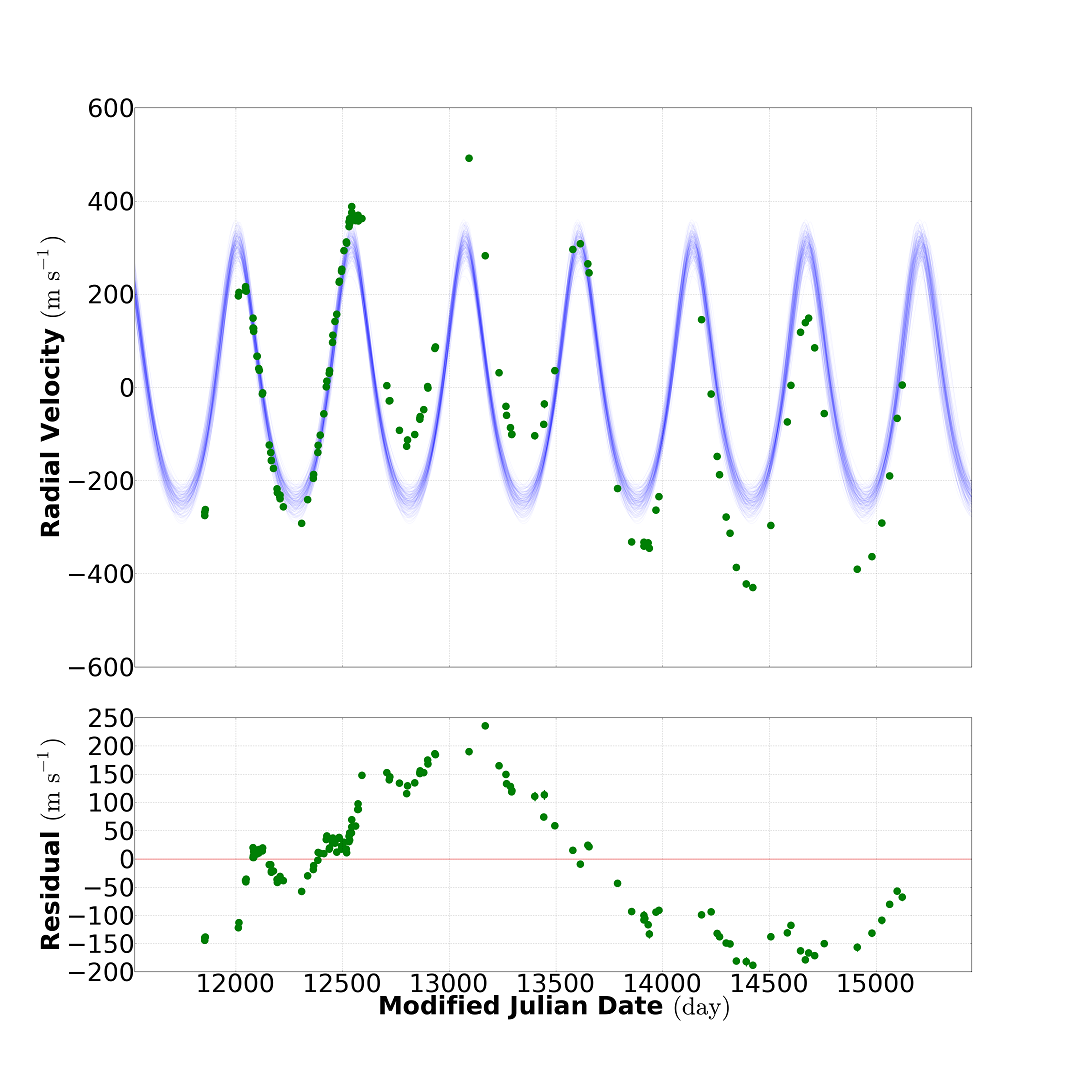
\includegraphics[width=0.49\linewidth]{fit_res_282_mod_1_20130930_.png}} &
	\subfloat[2-Companion Model]{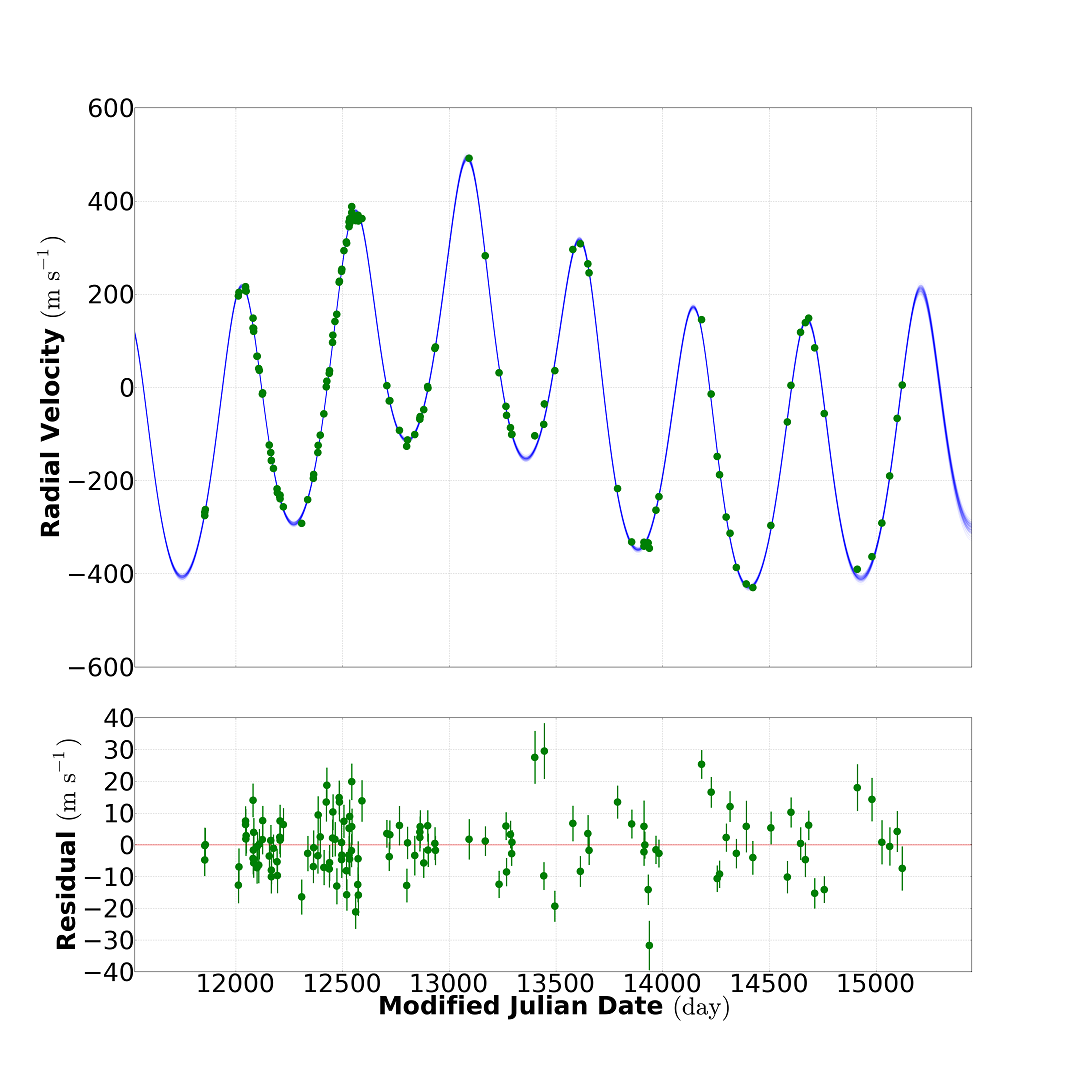
\includegraphics[width=0.49\linewidth]{fit_res_282_mod_2_20130930_.png}} \\
	\subfloat[3-Companion Model]{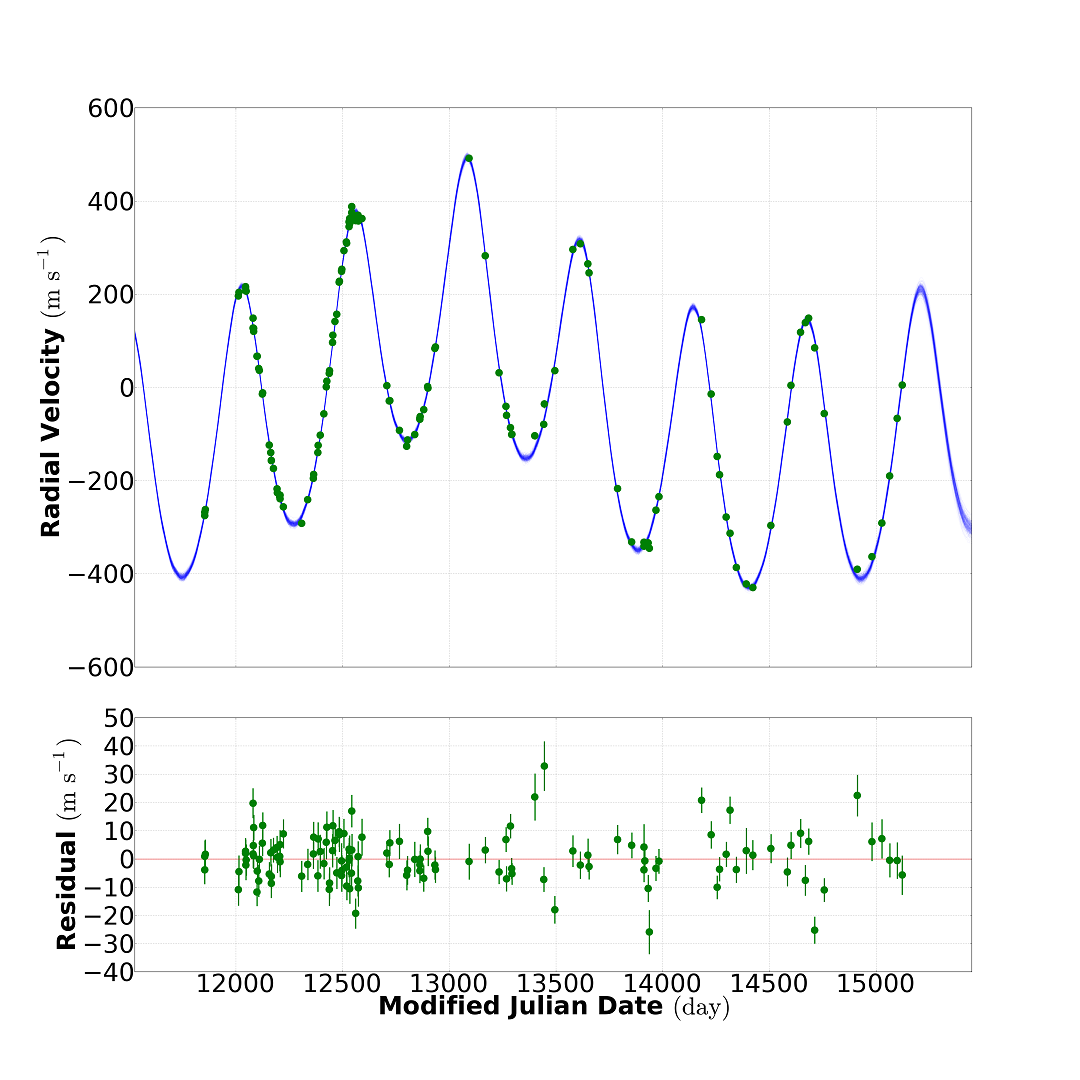
\includegraphics[width=0.49\linewidth]{fit_res_282_mod_3_20130930_.png}} &
	\subfloat[4-Companion Model]{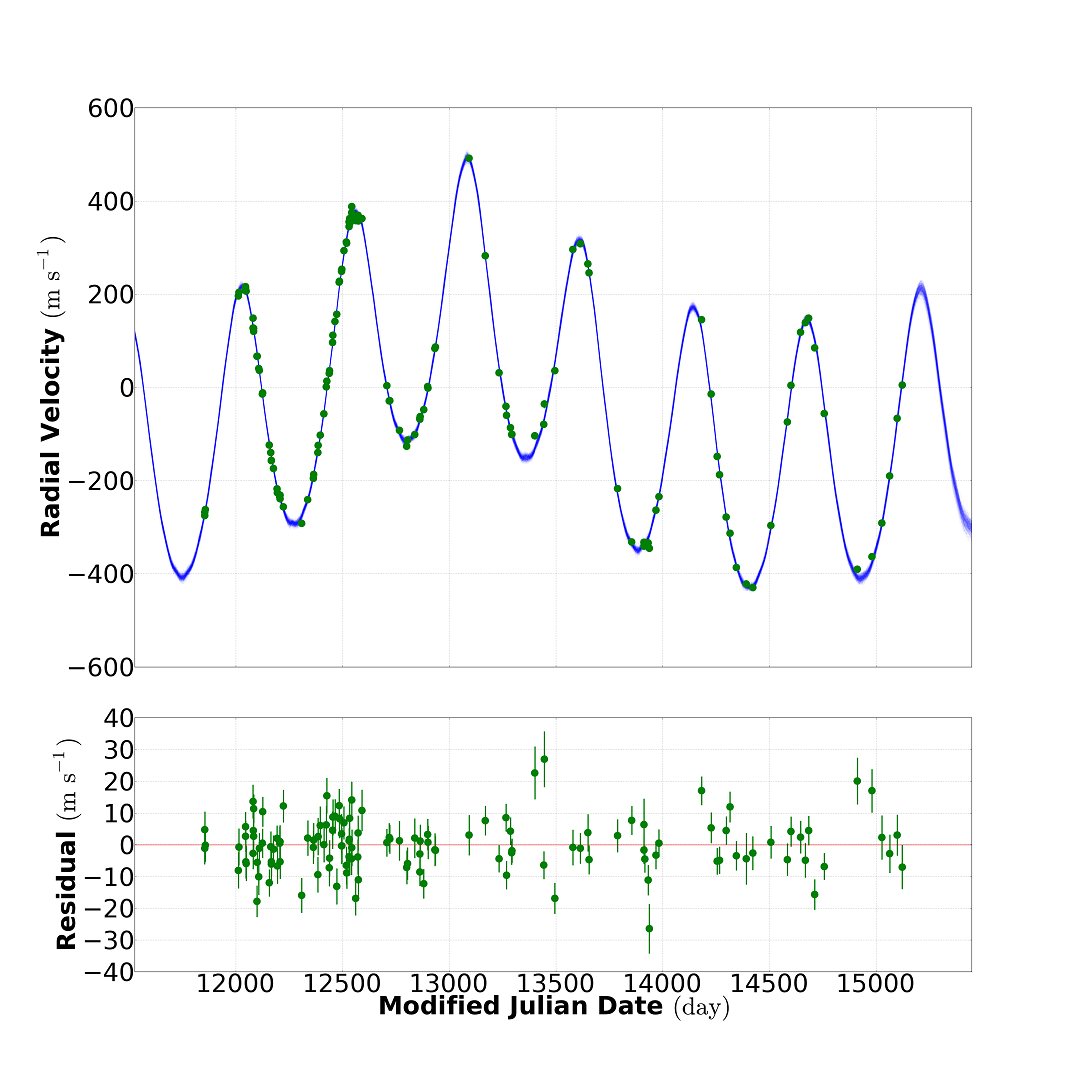
\includegraphics[width=0.49\linewidth]{fit_res_282_mod_4_20130930_.png}}
 \end{tabular}
 \caption{(a) In the upper panel, the blue lines show 100 sample fits from the posterior probability distribution of the 1-companion model, and the green dots show the data. In the bottom panel, the residual data for the best fit of the 1-companion model are shown. (b) In the upper panel, data and 100 sample fits from the posterior probability distribution of the 2-companion model are shown. In the bottom panel. The residual data are shown. (c) In the upper panel, data and 100 sample fits from the posterior probability distribution of the 3-companion model are shown. In the bottom panel. The residual data are shown. (d) In the upper panel, data and 100 sample fits from the posterior probability distribution of the 4-companion model are shown. In the bottom panel. The residual data are shown.}
 \label{fig:282-fits}
\end{figure}

\begin{comment}

\begin{figure}
 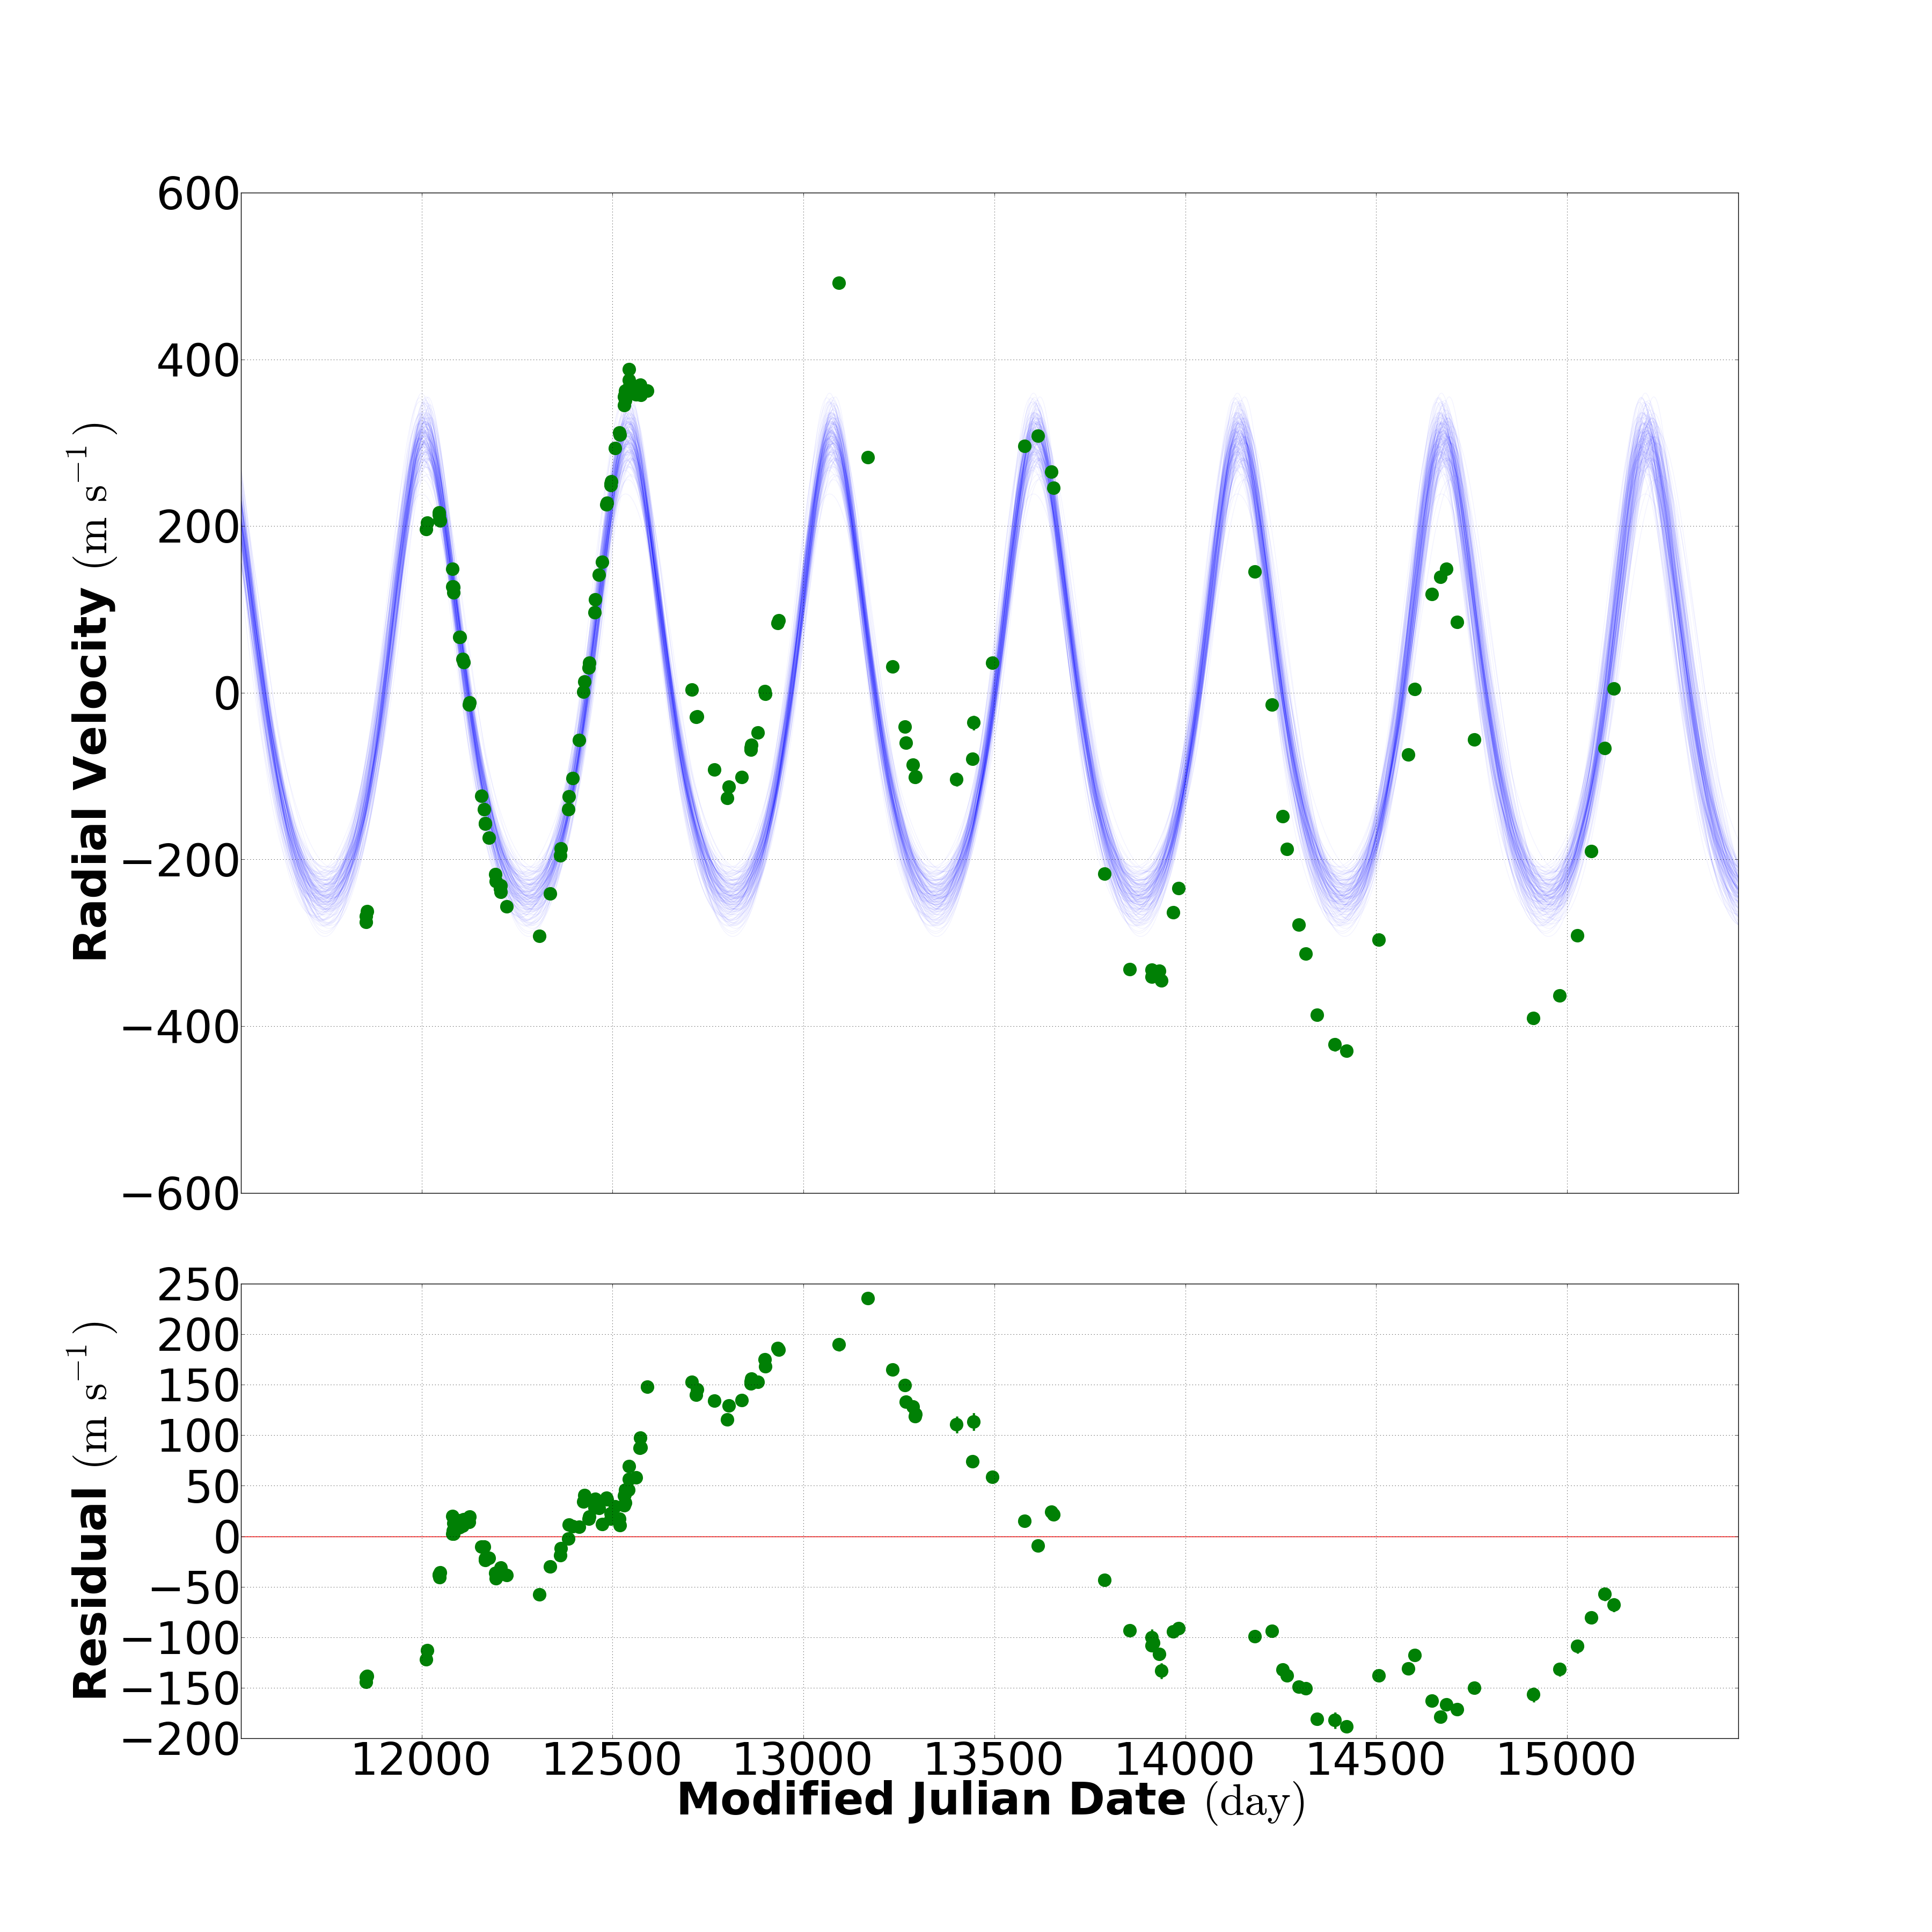
\includegraphics[width=0.99\linewidth]{fit_res_282_mod_1_20130930.png}
 \caption{The top panel shows the RV data for HIP 88048 and 100 sample fits from the posterior of 1-companion model. The bottom panel shows the residual data for the best fit among them.}
 \label{fig:282-1-fit}
\end{figure}

\begin{figure}
 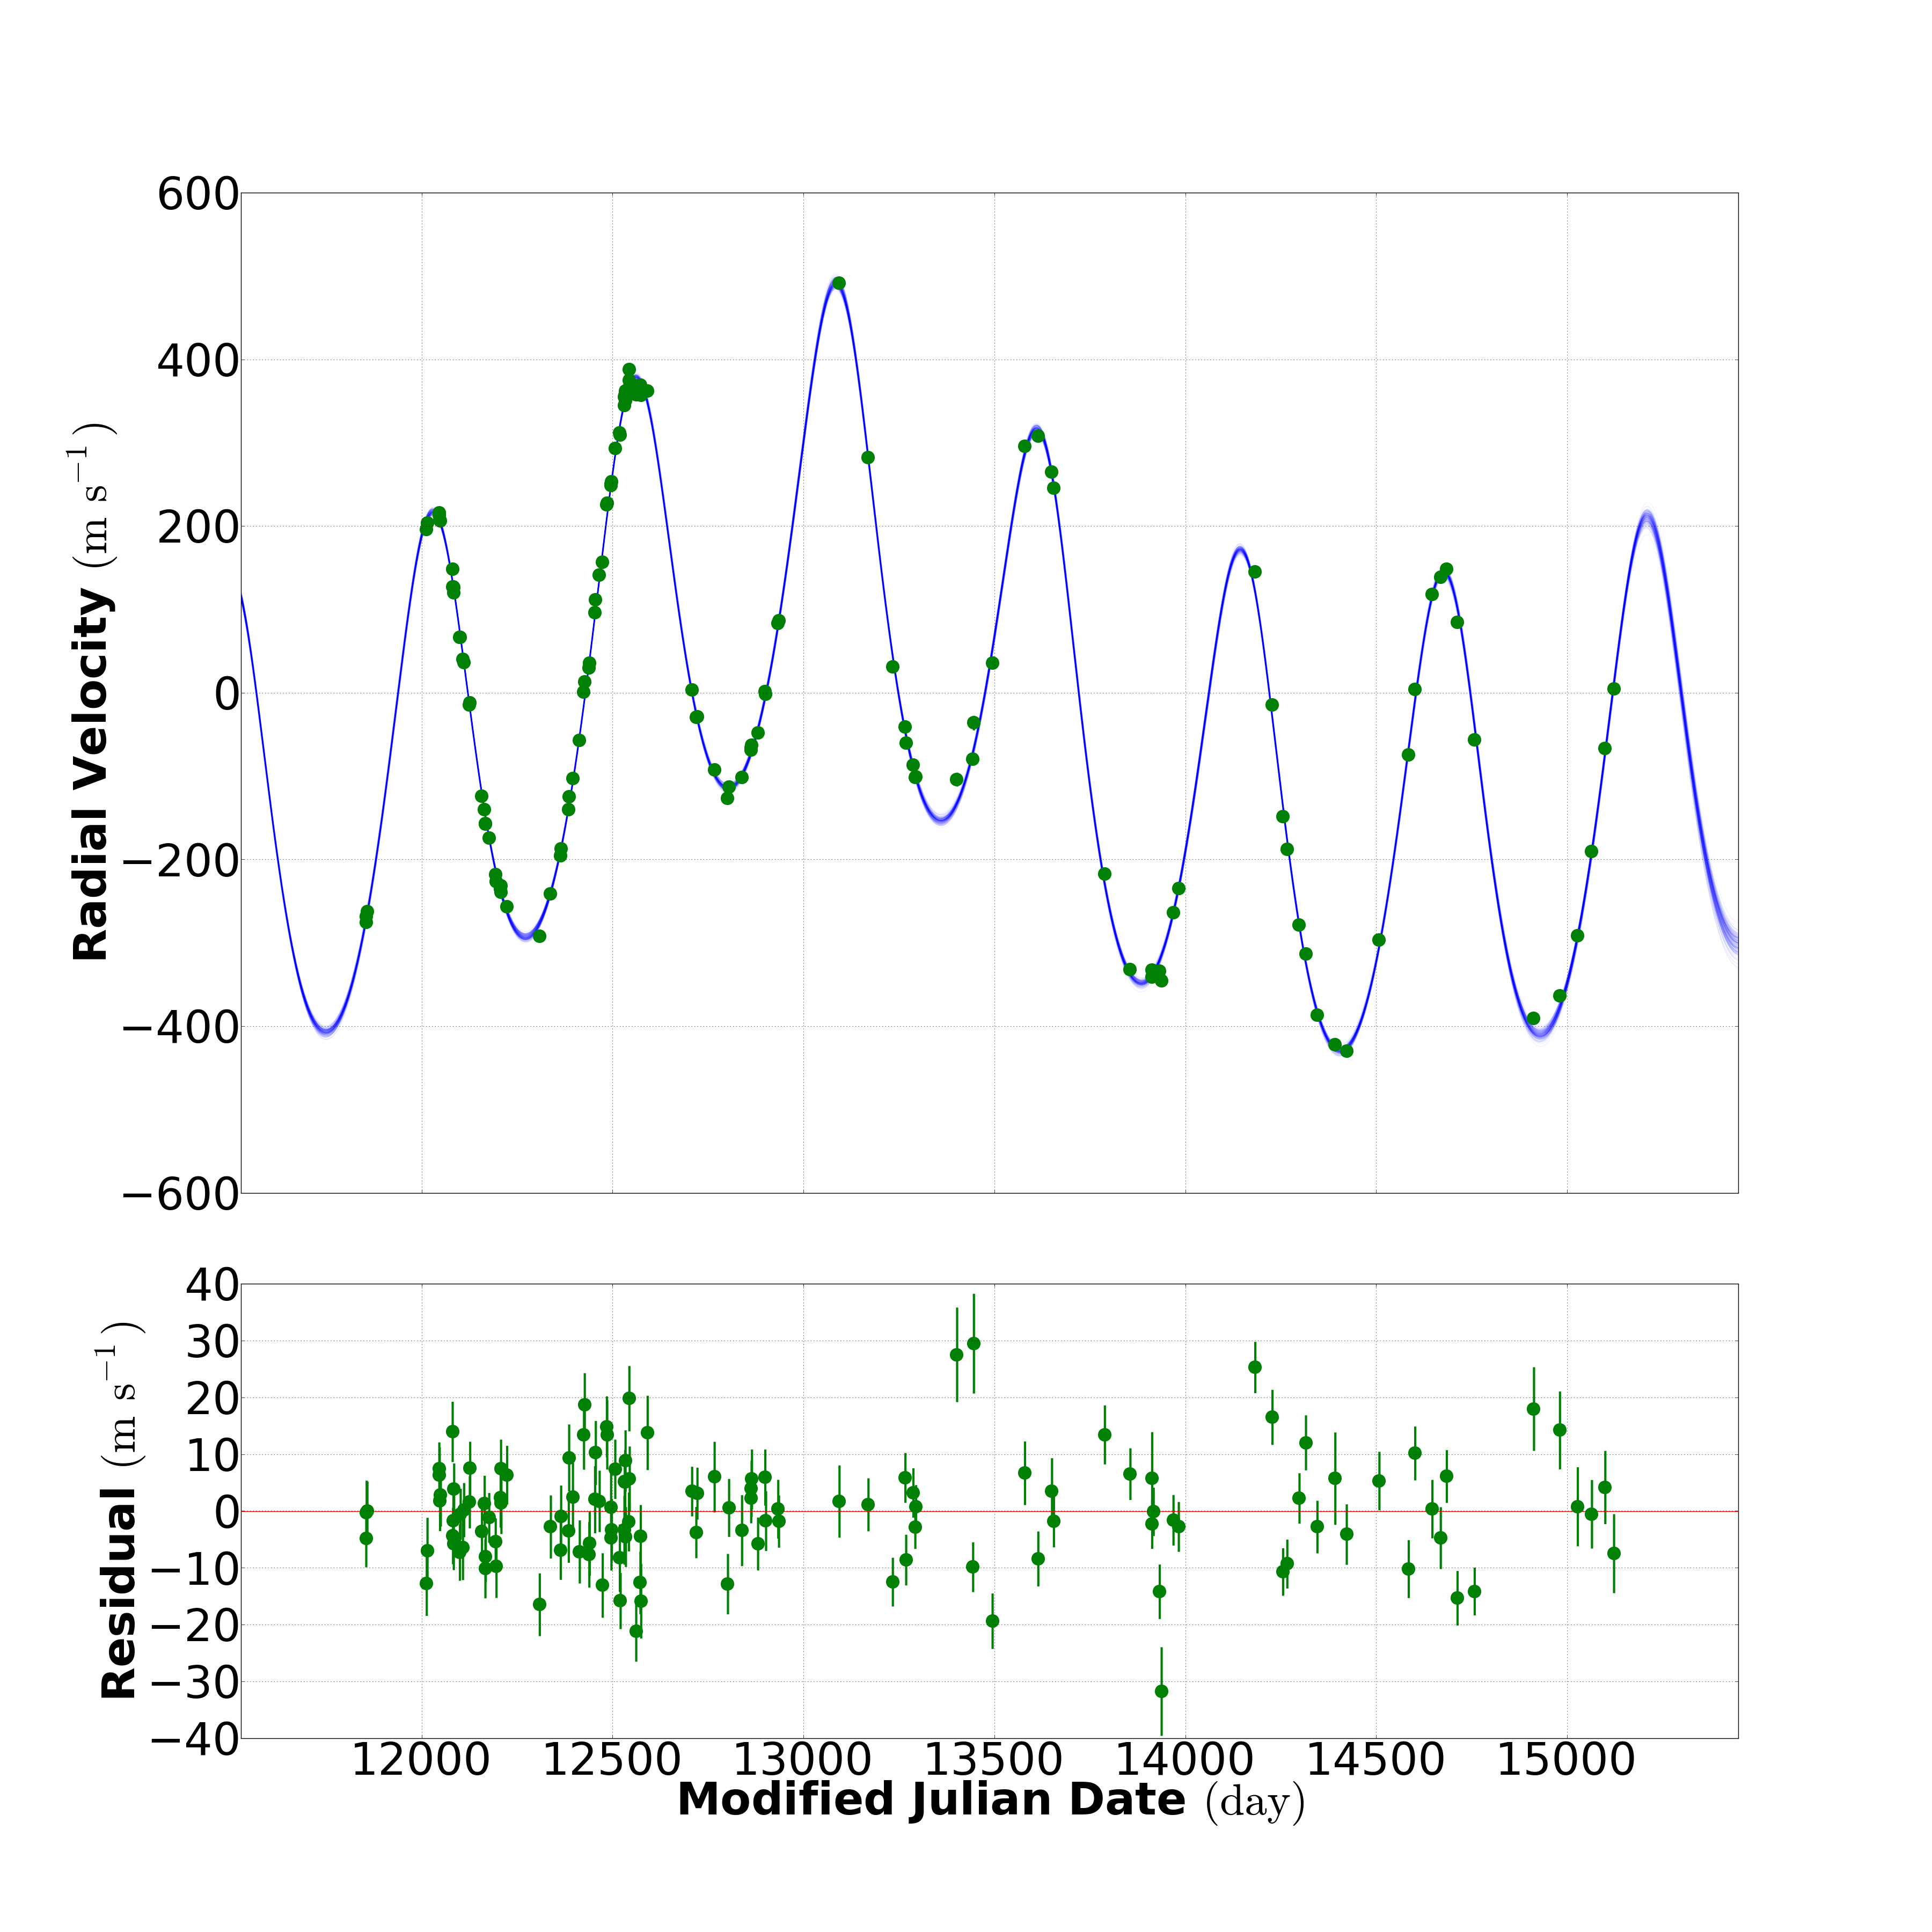
\includegraphics[width=0.99\linewidth]{fit_res_282_mod_2_20130930.png}
 \caption{The top panel shows the RV data for HIP 88048 and 100 sample fits from the posterior of 2-companion model. The bottom panel shows the residual data for the best fit among them.}
 \label{fig:282-2-fit}
\end{figure}

\begin{figure}
 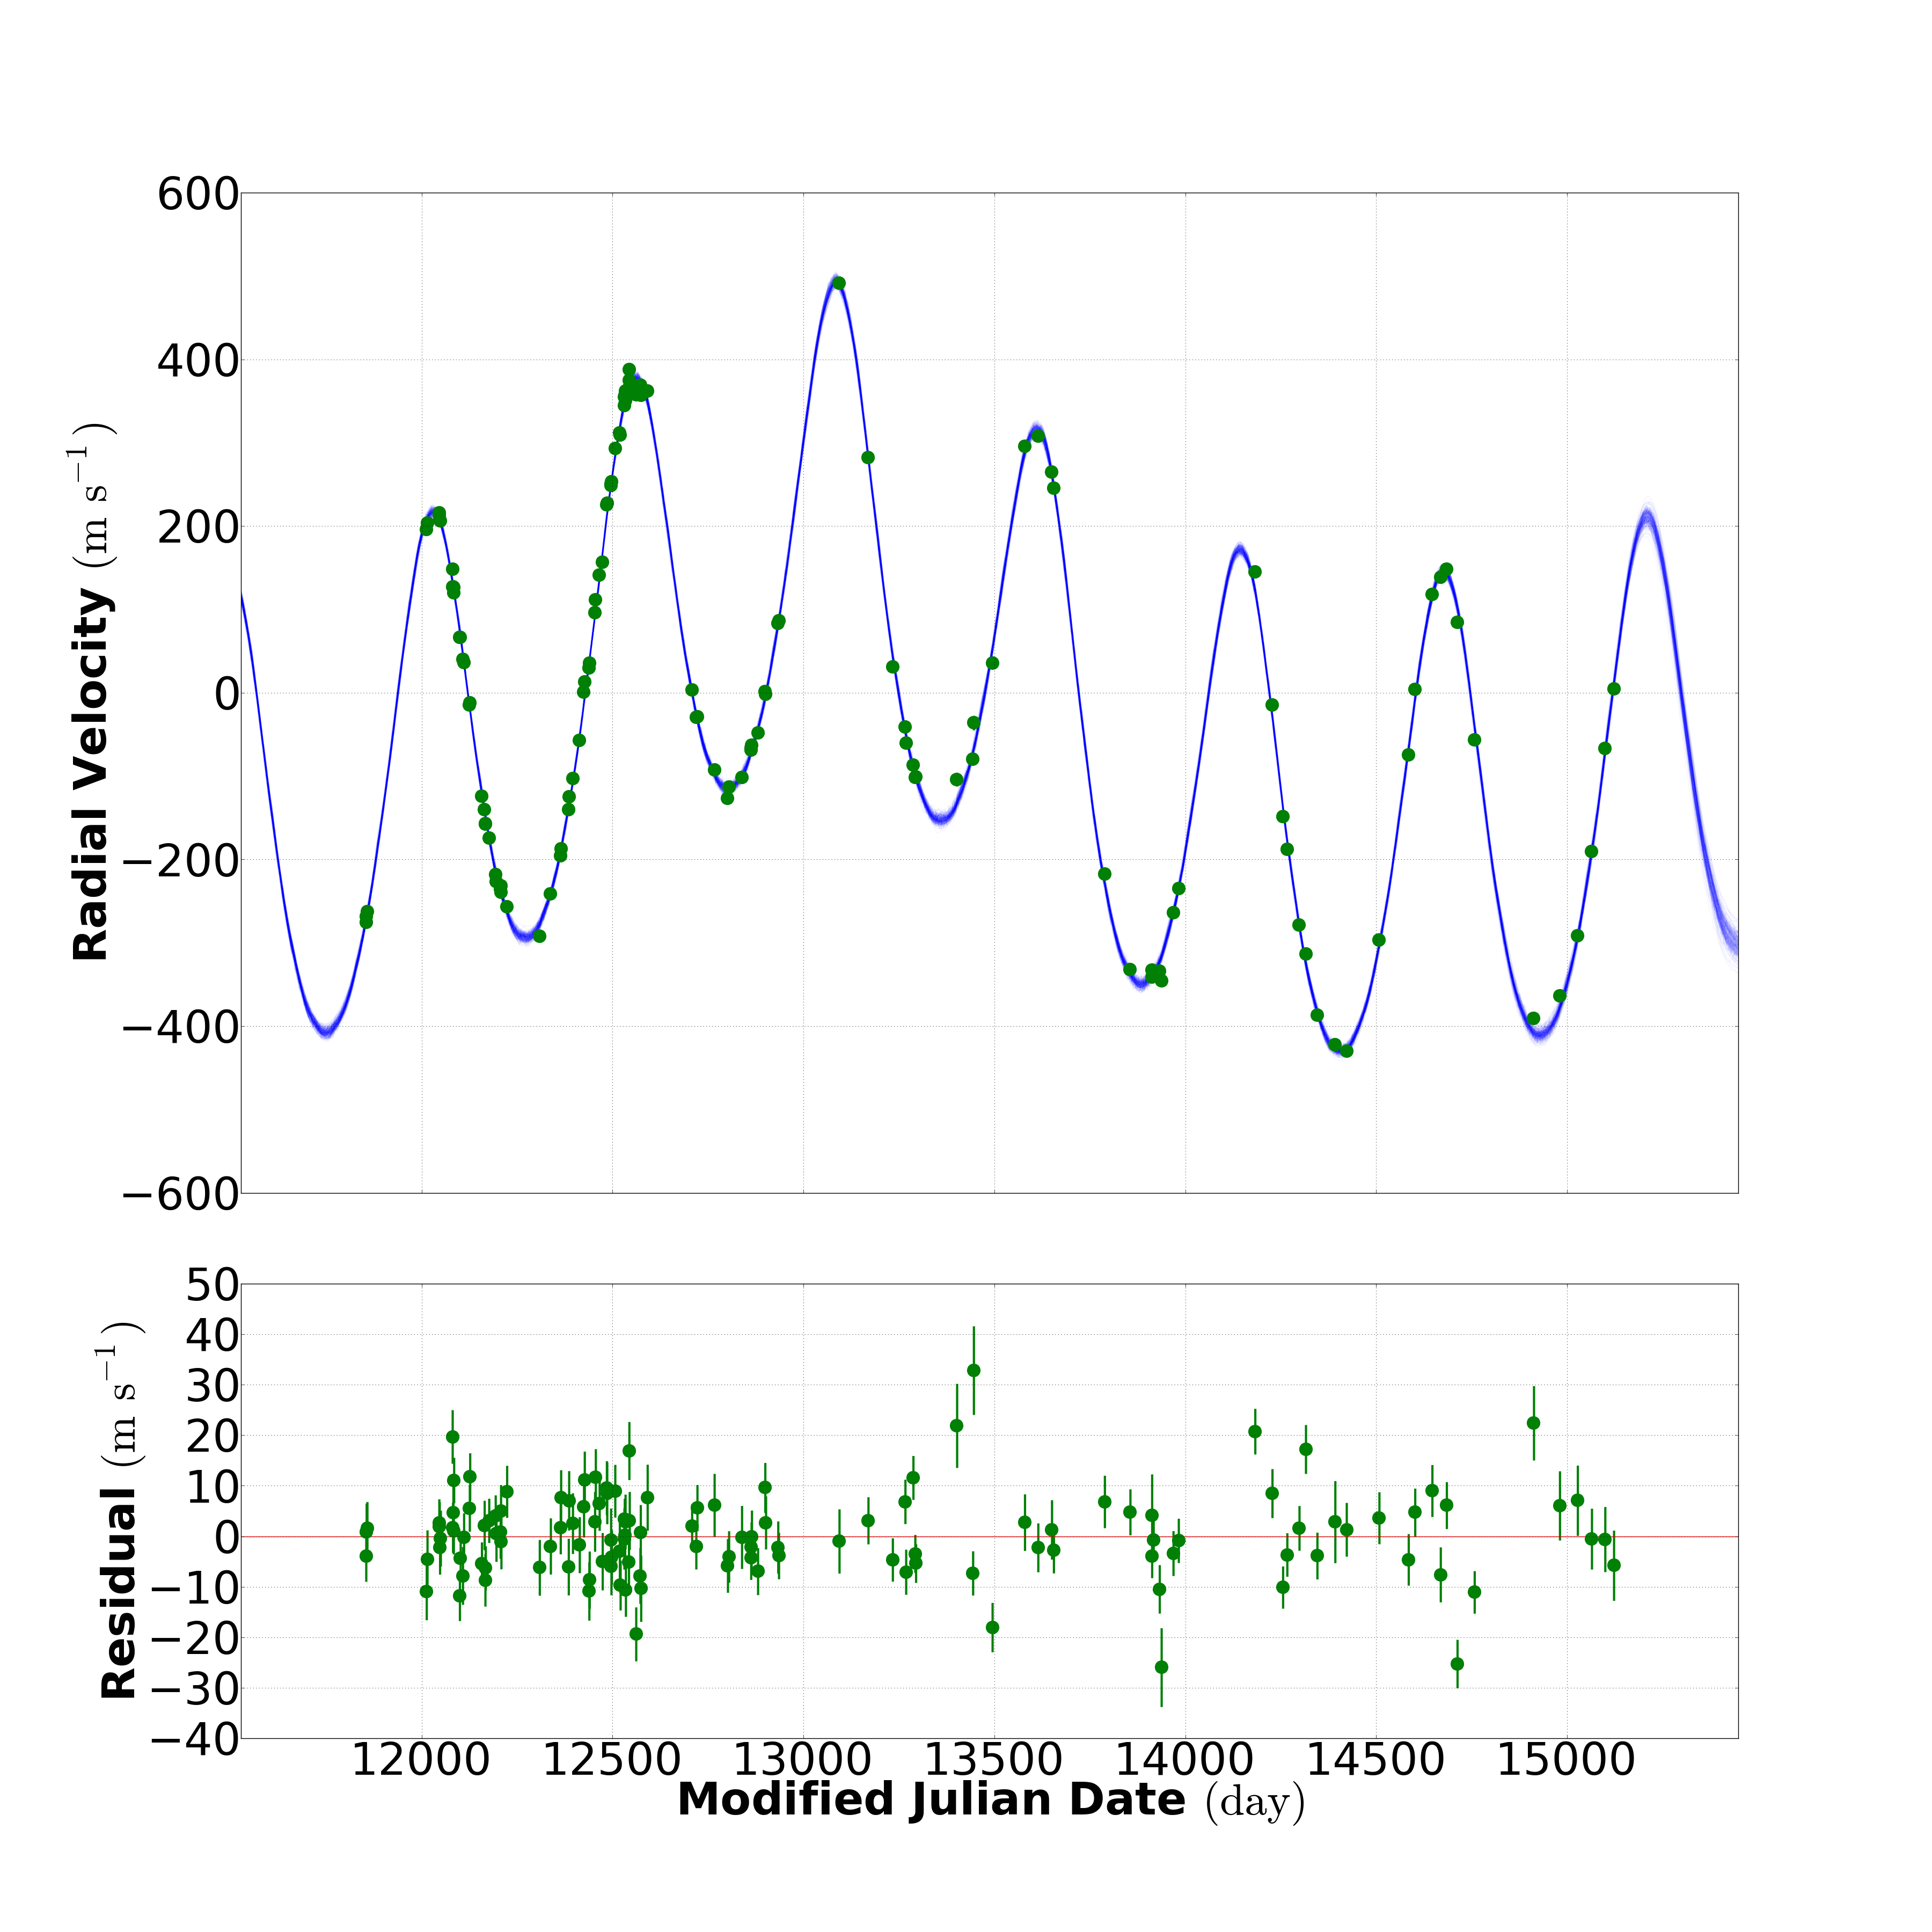
\includegraphics[width=0.99\linewidth]{fit_res_282_mod_3_20130930.png}
 \caption{The top panel shows the RV data for HIP 88048 and 100 sample fits from the posterior of 3-companion model. The bottom panel shows the residual data for the best fit among them.}
 \label{fig:282-3-fit}
\end{figure}

\begin{figure}
 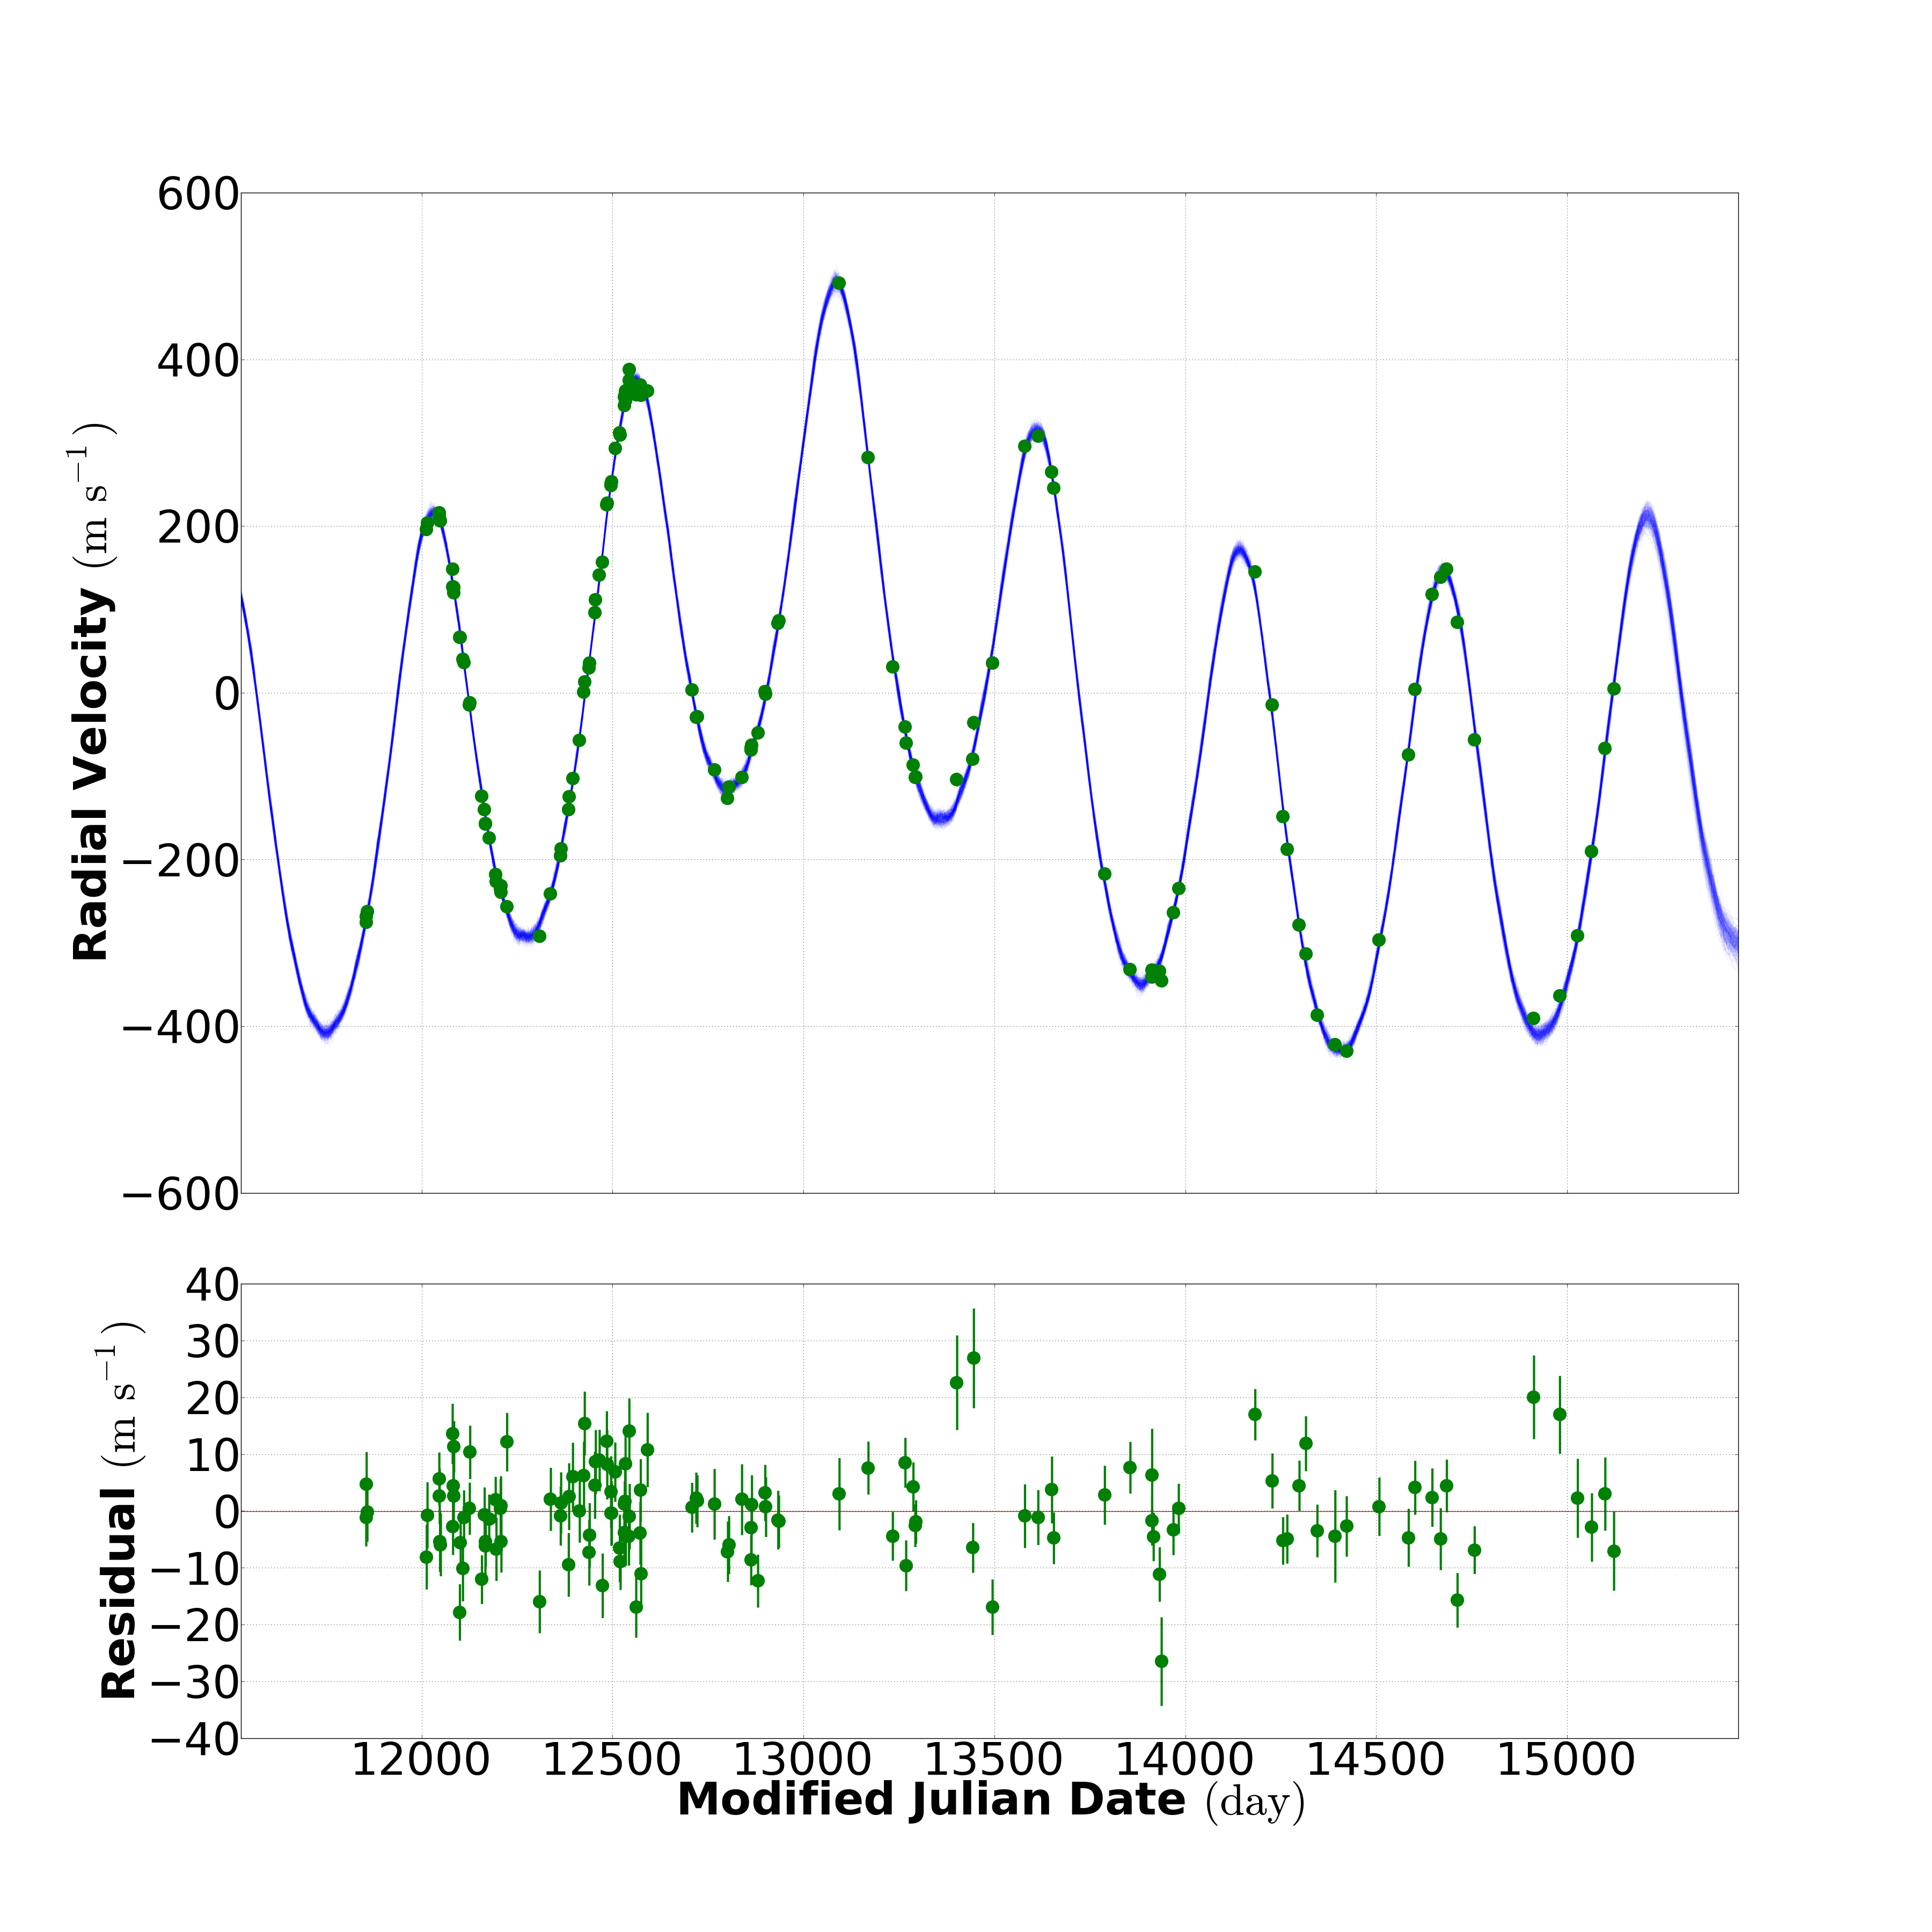
\includegraphics[width=0.99\linewidth]{fit_res_282_mod_4_20130930.png}
 \caption{The top panel shows the RV data for HIP 88048 and 100 sample fits from the posterior of 4-companion model. The bottom panel shows the residual data for the best fit among them.}
 \label{fig:282-4-fit}
\end{figure}

\end{comment}

\begin{figure}
 \centering
 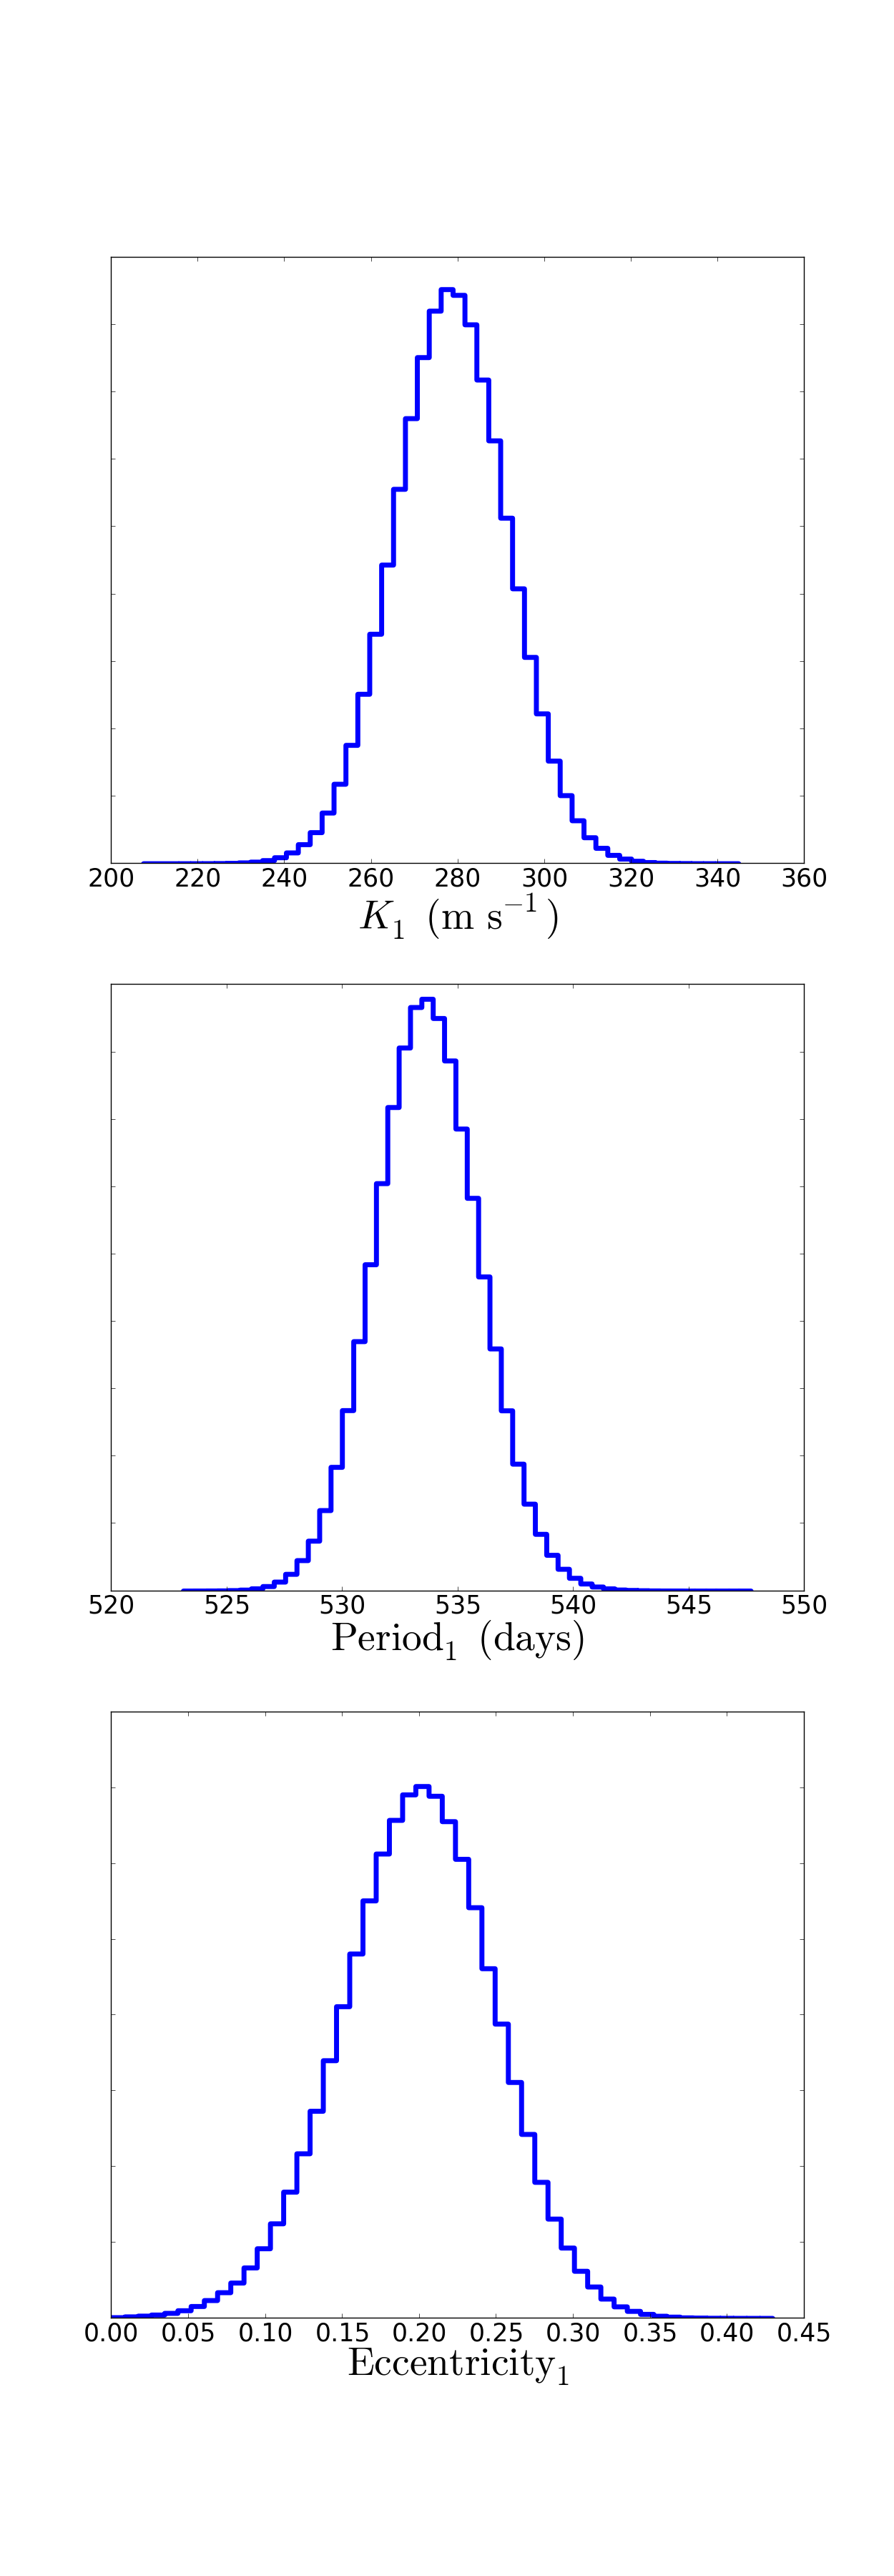
\includegraphics[width=0.45\linewidth]{282-1-hist.png}
 \caption{The posterior histograms of amplitude, period and eccentricity in the 1-companion model. All parameters are well constrained by the posterior distribution.}
 \label{fig:282-1-hist}
\end{figure}

\begin{figure}
 \centering
 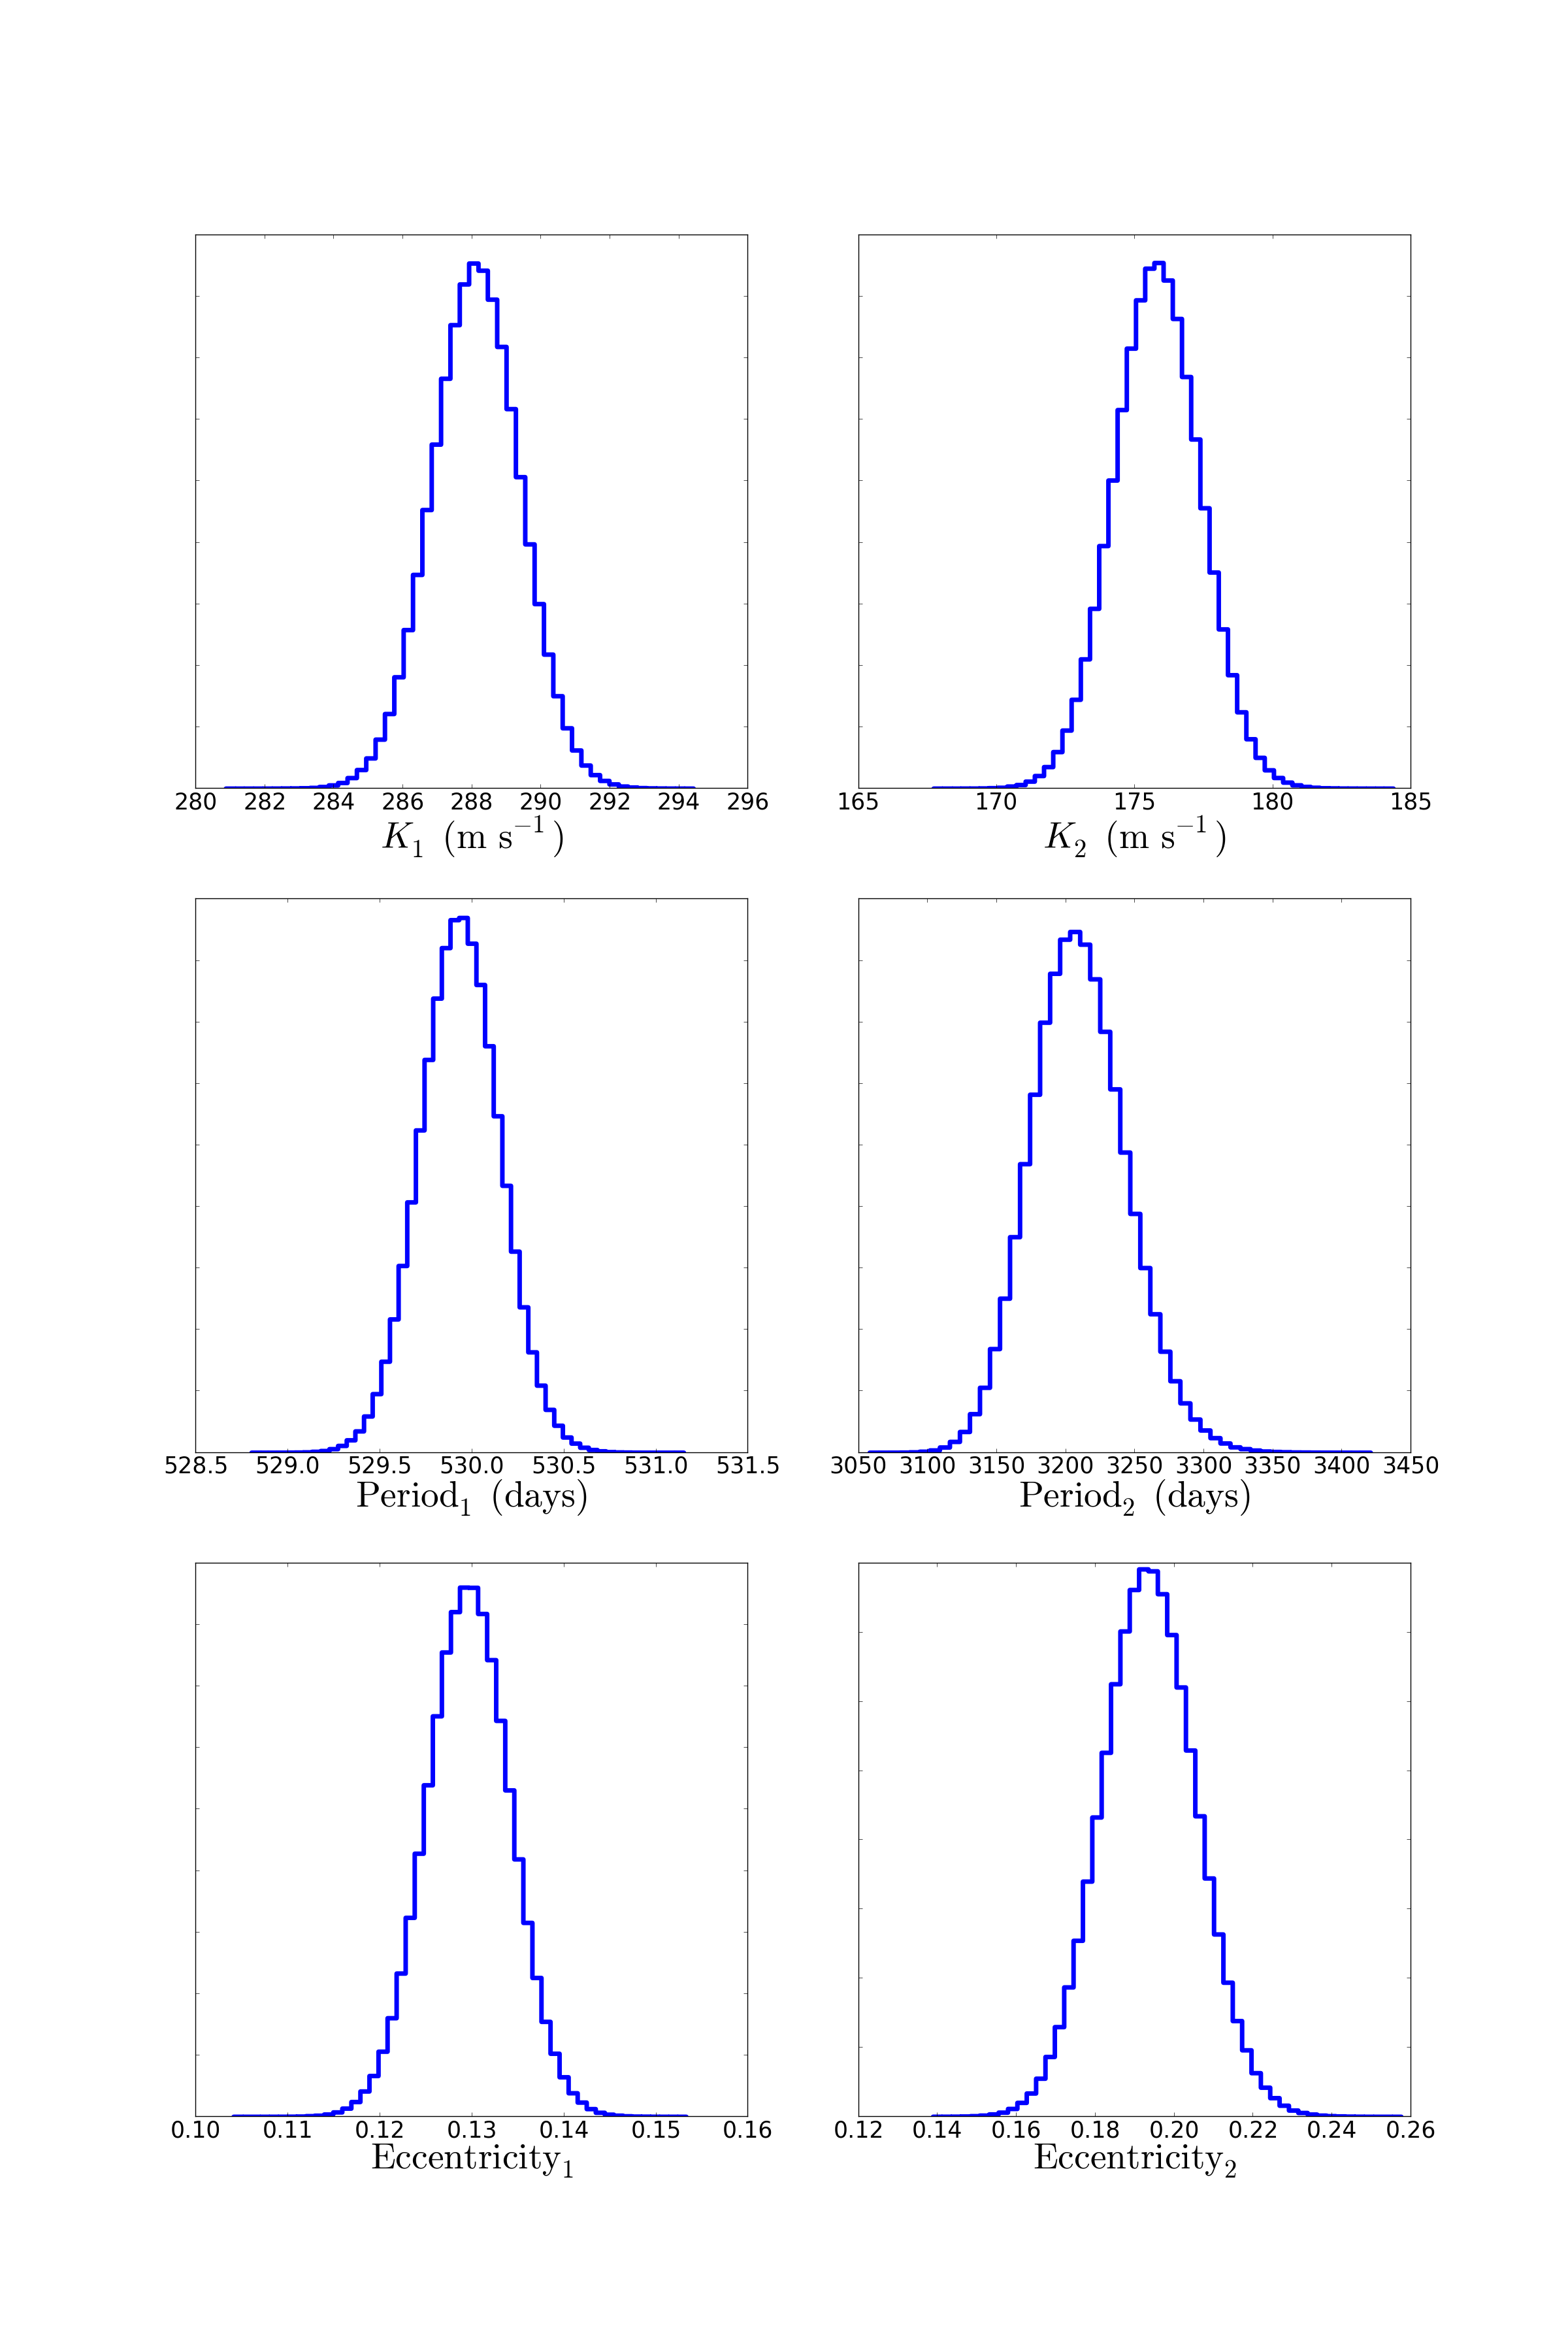
\includegraphics[width=0.80\linewidth]{282-2-hist.png}
 \caption{The posterior histograms of amplitudes, periods and eccentricities of both the companions in the 2-companion model. All the parameters are well constrained by the posterior distribution.}
 \label{fig:282-2-hist}
\end{figure}

\begin{figure}
 \centering
 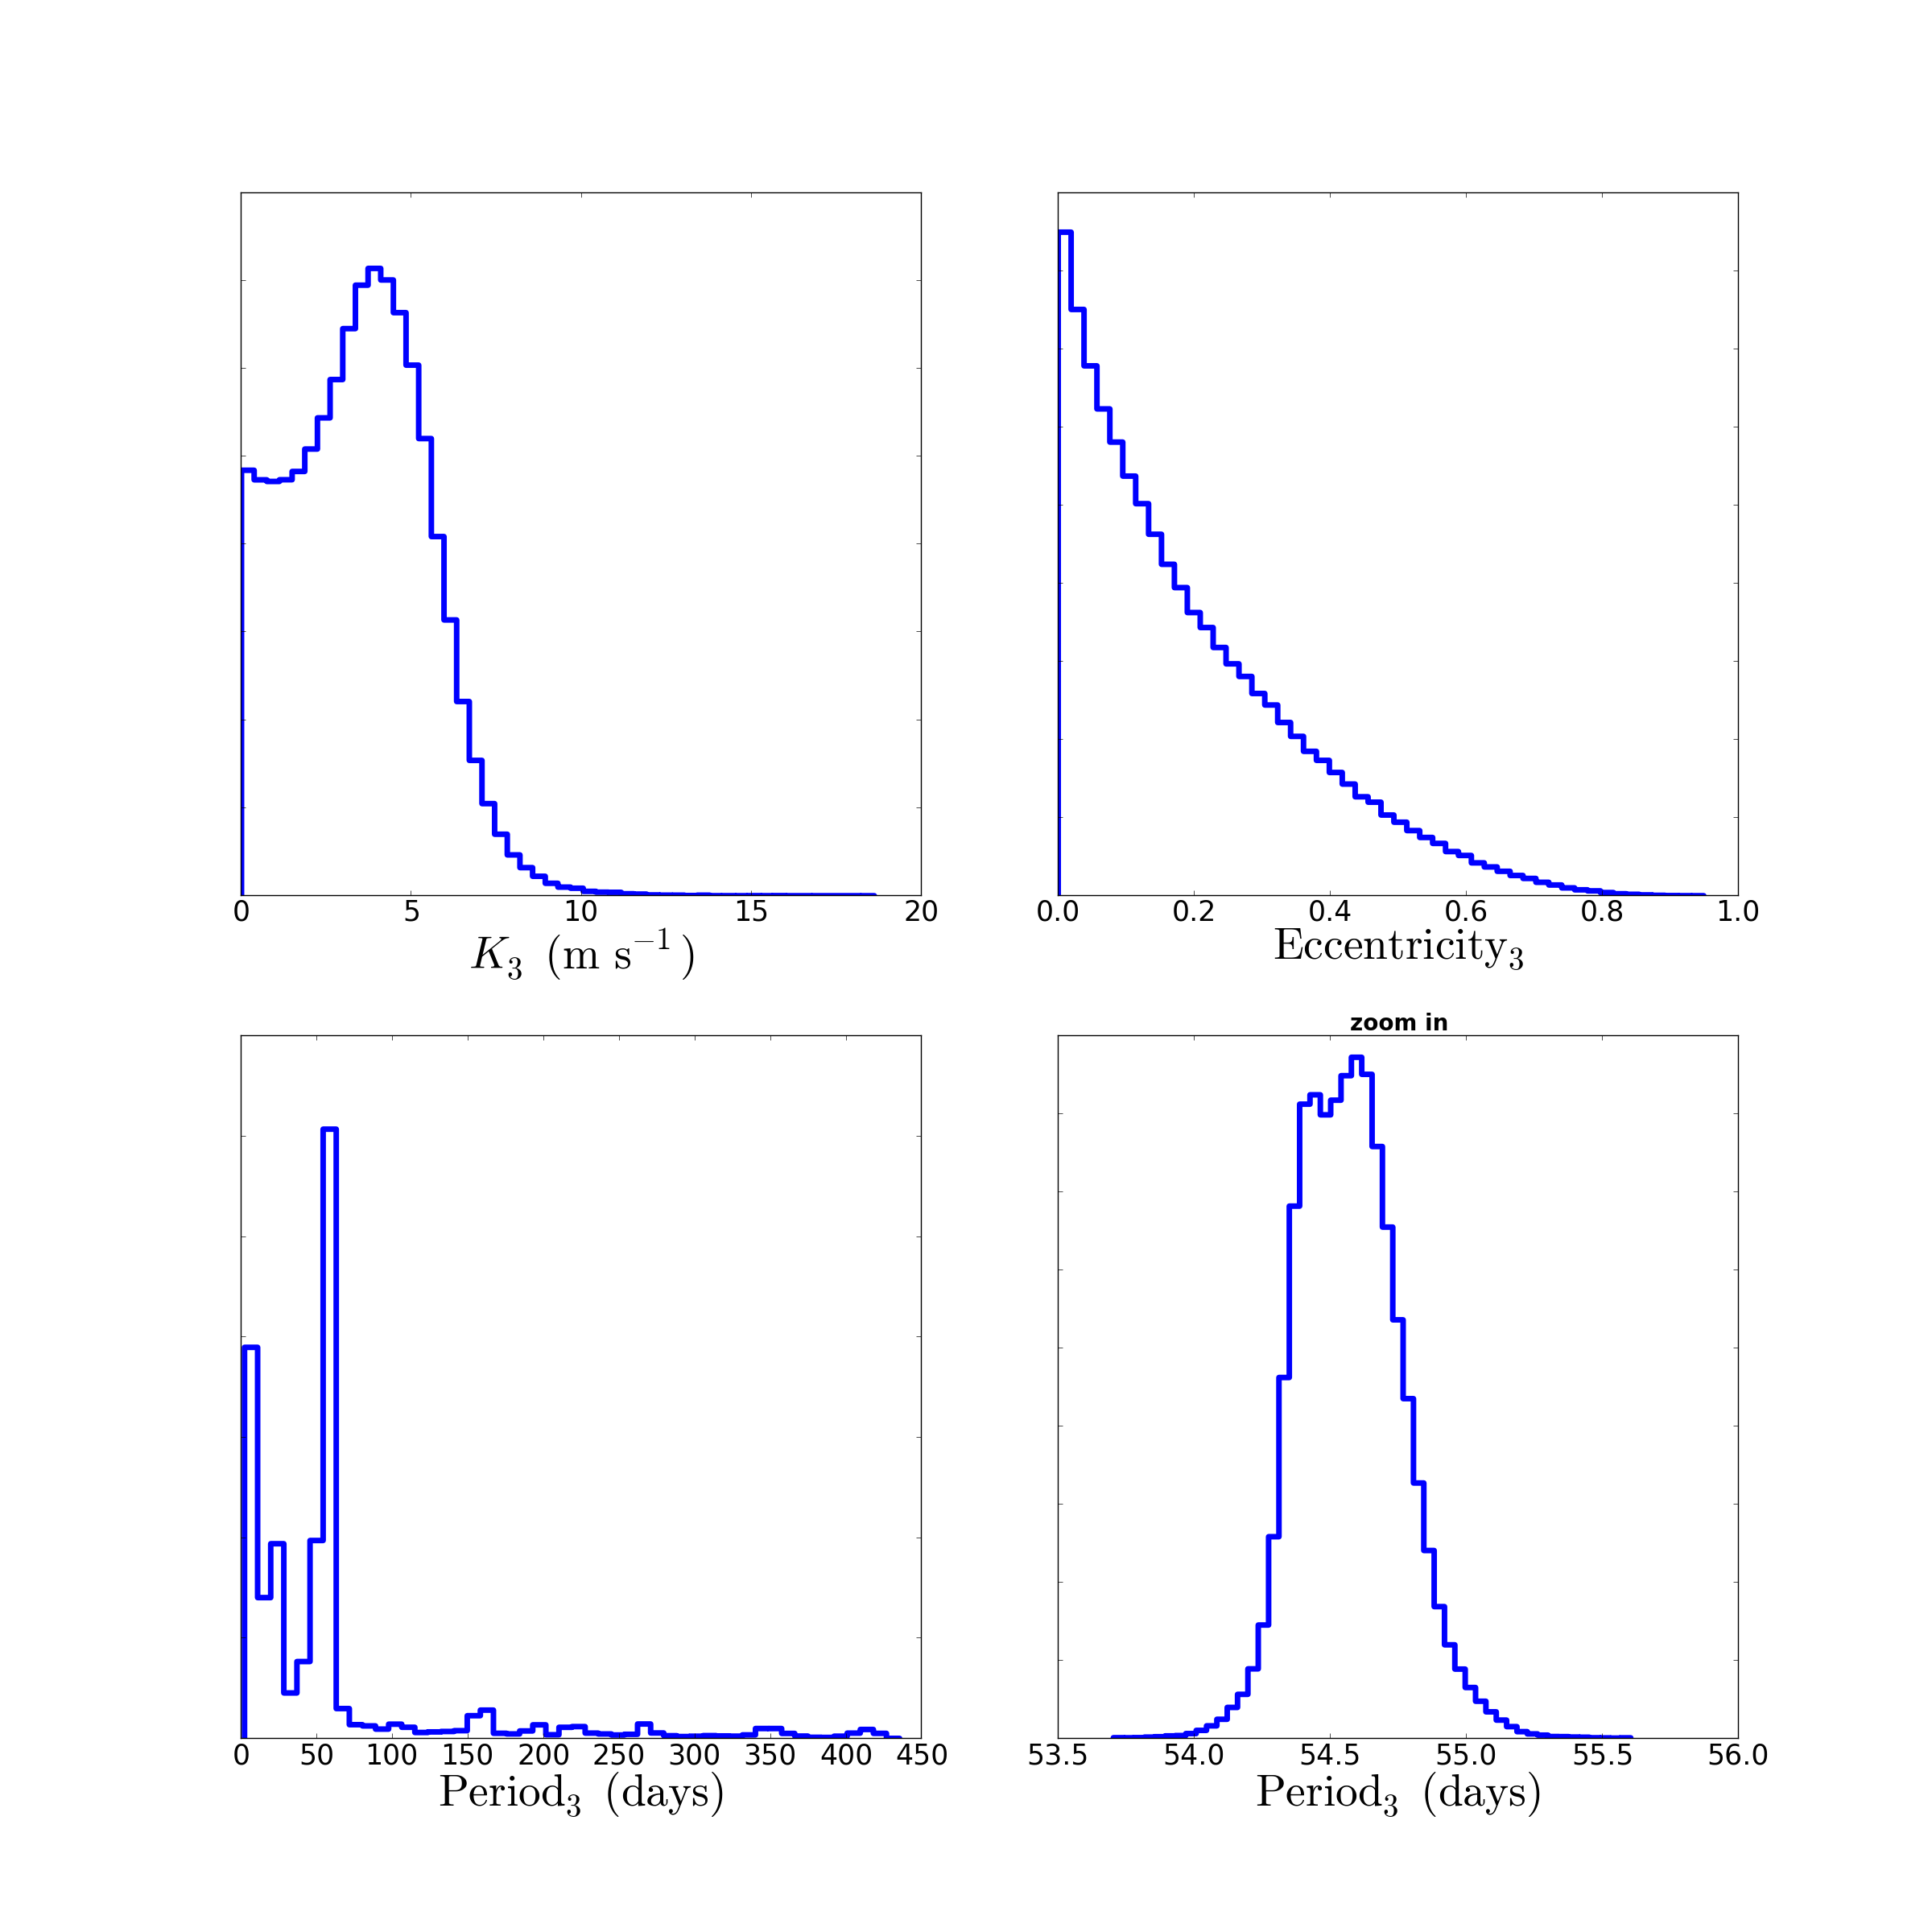
\includegraphics[width=0.99\linewidth]{282-3-hist.png}
 \caption{The posterior histograms of amplitude, period and eccentricity of the 3rd companion in the 3-companion model. The histograms of the other 2 companions are almost identical to their histograms in 2-companion model, shown in Fig.~\ref{fig:282-2-hist}. The histogram of the amplitude indicates that small object is favored. The histogram of period indicates that the period of the 3rd companion is poorly constrained, but there are many peaks in the histogram. The histogram on the lower right side is for the period of the 3rd companion, but zoomed in around the peak of about 54 days. The histogram of the eccentricity shows that the data almost provides no information for eccentricity of the 3rd companion, and the posterior is very close to the prior for eccentricity given in Eqn.~(\ref{eq:prior-e}).}
 \label{fig:282-3-hist}
\end{figure}

\begin{figure}
 \centering
 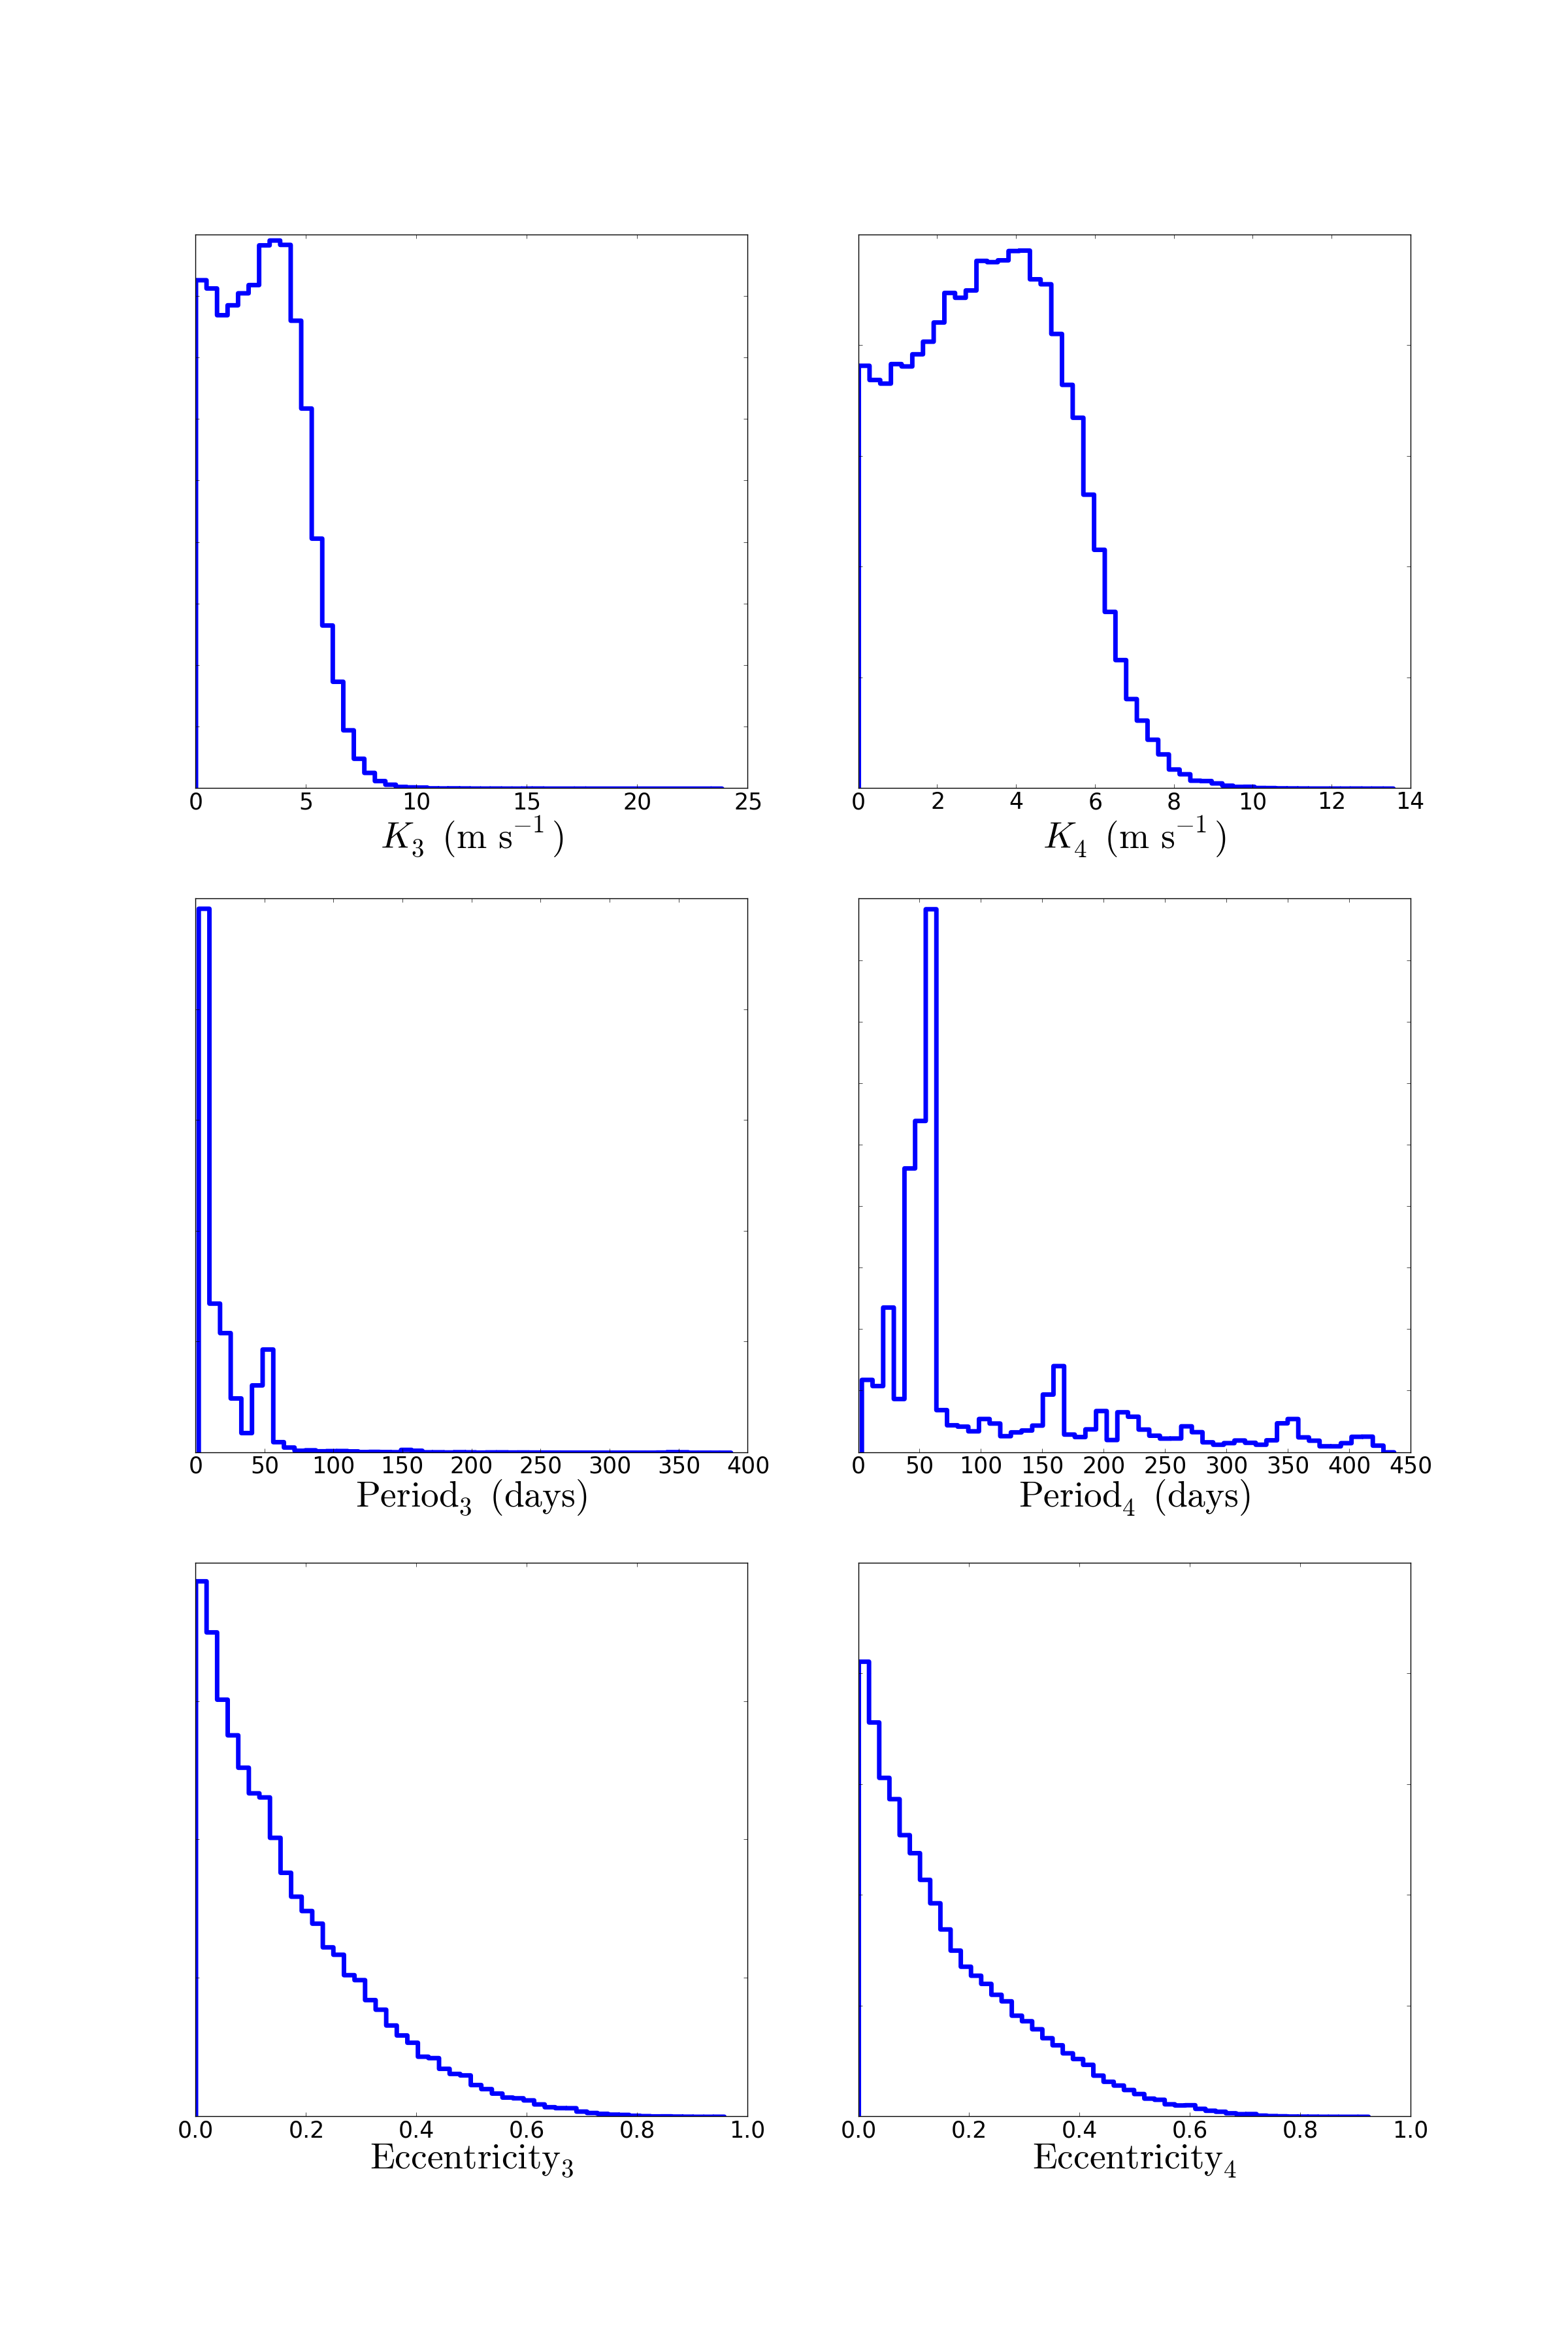
\includegraphics[width=0.80\linewidth]{282-4-hist.png}
 \caption{The posterior histograms of amplitudes, periods and eccentricities of the 3rd and 4th companion in the 4-companion model. The histograms of the other 2 companions are again almost identical to their histograms in 2-companion model, shown in Fig.~\ref{fig:282-2-hist}. The histograms of amplitudes indicate that both objects are small if they exist. The histograms of periods indicate that the periods are poorly constrained but they do show various peaks, including a peak around 54 days. The histograms of eccentricities are both very similar to the prior for eccentricity given in Eqn.~(\ref{eq:prior-e}).}
 \label{fig:282-4-hist}
\end{figure}

\end{document}
